\chapter{System Overview}

This chapter presents the PawPal system architecture, data design, domain models, and detailed design diagrams. The system employs a modular monolithic backend (Golang), cross-platform mobile frontend (Flutter), and specialized AI services (Python) with layered architecture for separation of concerns.

\section{Architectural Design}

The system uses a three-tier architecture: presentation tier (Flutter mobile app), business logic tier (Golang backend with eight modules), and data tier (PostgreSQL with Redis caching). AI services run as isolated Python microservices for efficient ML framework integration.

\subsection{High-Level Architecture}

The system architecture can be visualized as a client-server model with the following major components:

\begin{figure}[H]
    \centering
    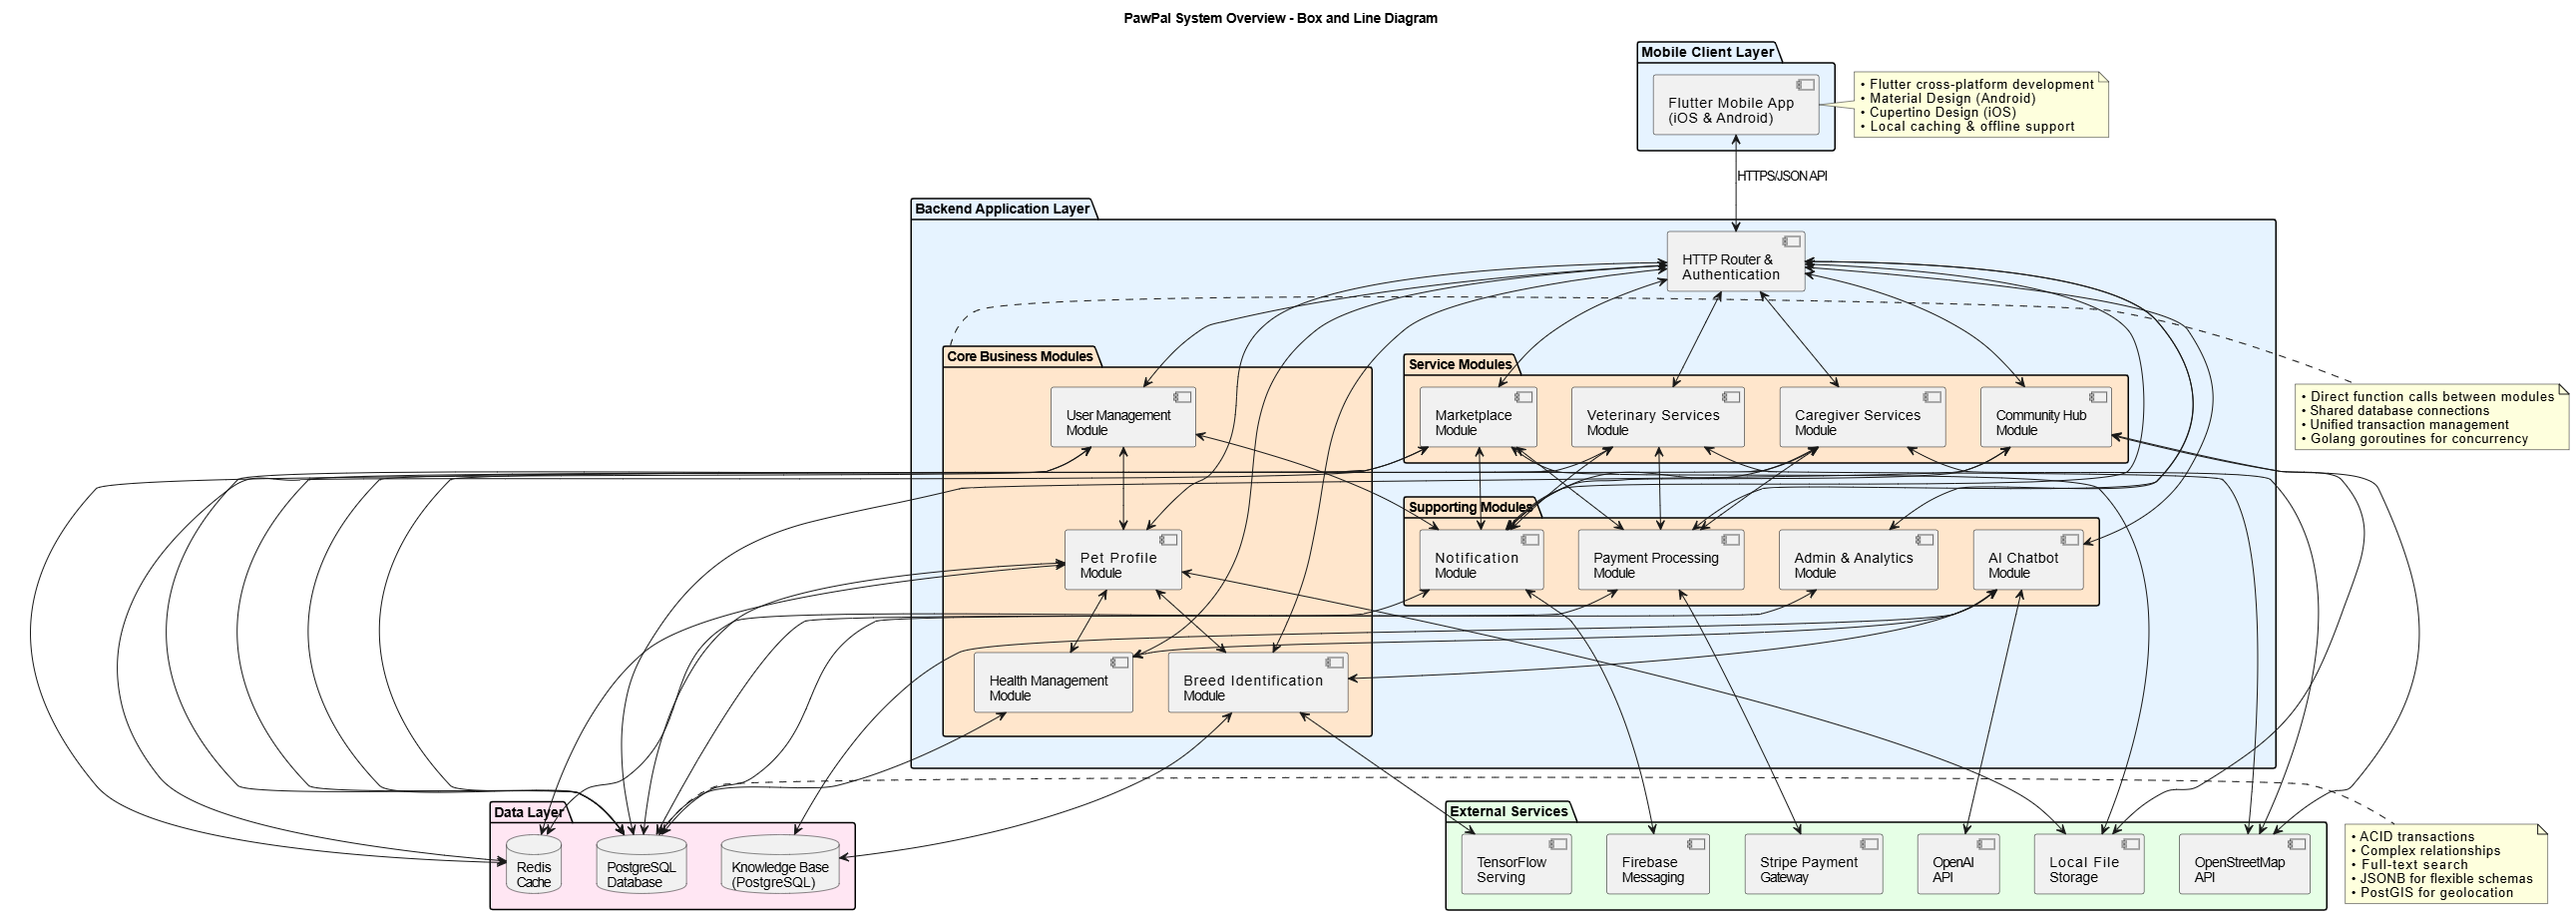
\includegraphics[width=1.0\textwidth]{ThesisFigs/system_overview_box_line.png}
    \caption{PawPal System Overview - Box and Line Diagram}
    \label{fig:system_overview}
\end{figure}

\textbf{Client Tier:} Flutter mobile app (iOS/Android) with Provider/Riverpod state management, SQLite offline persistence, HTTP client for API communication, and Firebase Cloud Messaging.

\textbf{API Gateway Tier:} Golang Gin framework with JWT authentication, rate limiting (100 req/min), request validation, and CORS configuration.

\textbf{Business Logic Tier (8 Modules):} Pet Identification (CNN inference), Chatbot (RAG pipeline), Pet Profiles \& Journals (health data), Marketplace (e-commerce), Community Hub (social features), Veterinary Services (appointments), Caregiver Services (provider management), Payment Integration (multi-currency).

\textbf{AI Services Tier:} FastAPI chatbot server (port 8000), ChromaDB vector database (281,438 docs), Groq llama-3.3-70b-versatile LLM, TensorFlow ConvNeXt V2 CNN, sentence transformers (all-MiniLM-L6-v2).

\textbf{Data Tier:} PostgreSQL 14+ (relational), Redis (caching/sessions), ChromaDB (vector embeddings), cloud storage (media files).

\textbf{External Services:} Groq API (LLM), OpenStreetMap (geolocation), Firebase (notifications), blockchain networks (cryptocurrency).

\subsection{Modular Monolithic Architecture}

All eight modules deploy as a single unit with clear boundaries and interfaces. Benefits include direct function calls for performance, simplified deployment, centralized logging, atomic transactions, and lower infrastructure costs. Each module uses consistent layers: Handlers (HTTP), Services (business logic), Models (entities), Repositories (database access), and Utils (shared functions).

\subsection{Hybrid Architecture for AI Services}

The chatbot uses hybrid architecture with two modes: (1) Primary HTTP mode sends requests to FastAPI service (port 8000) with persistent RAG pipeline, achieving 2-3s response time, and (2) Fallback exec mode spawns Python process if FastAPI unavailable. Automatic health checks determine execution mode.

\subsection{Layered Architecture}

The five-tier layered architecture ensures separation of concerns: (1) Presentation Layer - Flutter UI with state management, (2) API Gateway Layer - RESTful routing with authentication, (3) Business Logic Layer - eight modules with business rules, (4) Data Access Layer - repository pattern with GORM abstraction, (5) Data Storage Layer - PostgreSQL, Redis, and vector database.

\begin{figure}[H]
    \centering
    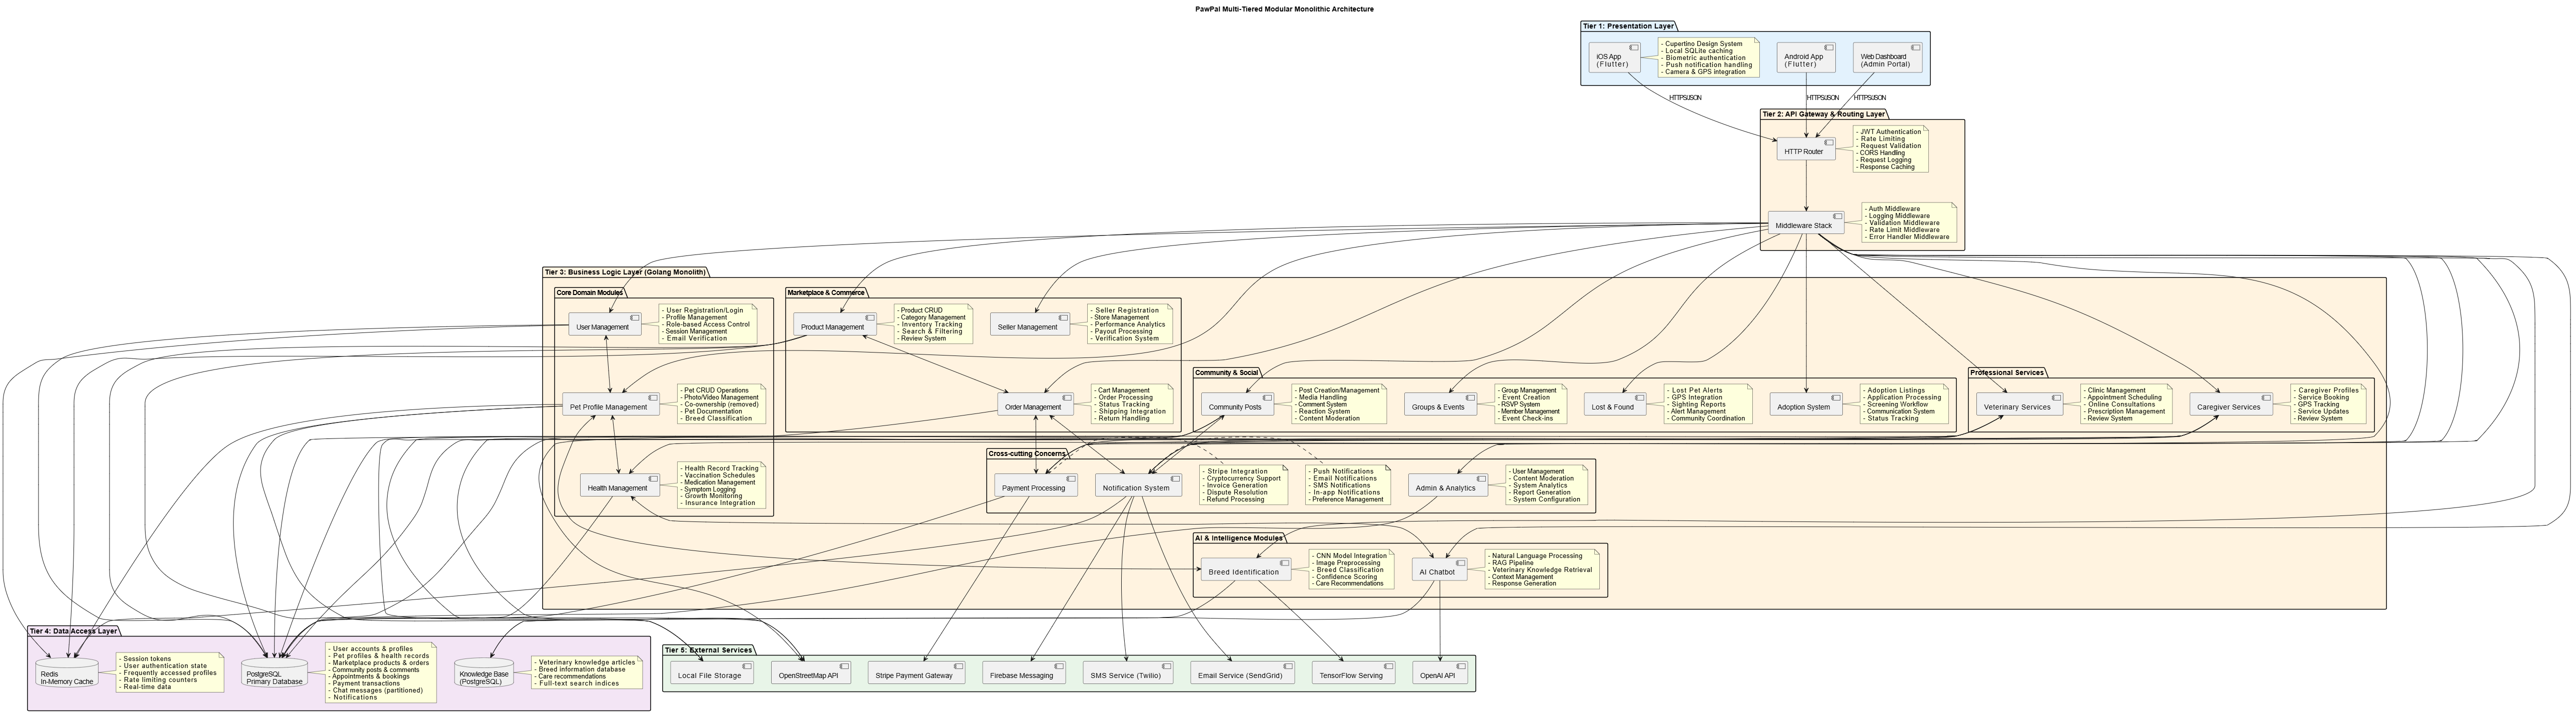
\includegraphics[width=1.0\textwidth]{ThesisFigs/layered_architecture.png}
    \caption{PawPal Detailed Layered Architecture}
    \label{fig:layered_architecture}
\end{figure}

\section{Data Design}

The data layer uses PostgreSQL (primary relational database), Redis (caching/sessions), and ChromaDB (vector embeddings). Schema design follows normalization principles with PostgreSQL JSONB for flexible metadata.

\subsection{Data Flow Diagrams}

The following data flow diagrams illustrate how data moves through the PawPal system across three levels of abstraction: Level 0 (context), Level 1 (main processes), and Level 2 (detailed sub-processes).

\subsubsection{Level 0: Context Diagram}

\begin{figure}[H]
    \centering
    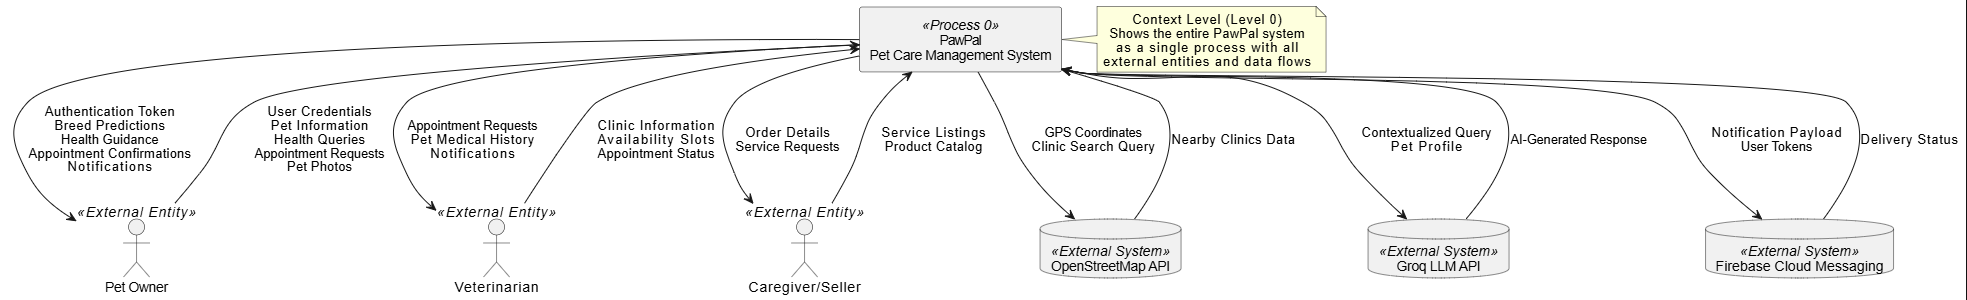
\includegraphics[width=0.95\textwidth]{ThesisFigs/dfd_level0.png}
    \caption{DFD Level 0: PawPal System Context Diagram showing external entities and data flows}
    \label{fig:dfd_level0}
\end{figure}

The context diagram shows the PawPal system as a single process interacting with three external entities (Pet Owner, Veterinarian, Caregiver/Seller) and three external systems (OpenStreetMap API, Groq LLM API, Firebase Cloud Messaging). Data flows include user credentials, pet information, health queries, breed predictions, and notifications.

\subsubsection{Level 1: Main Processes}

\begin{figure}[H]
    \centering
    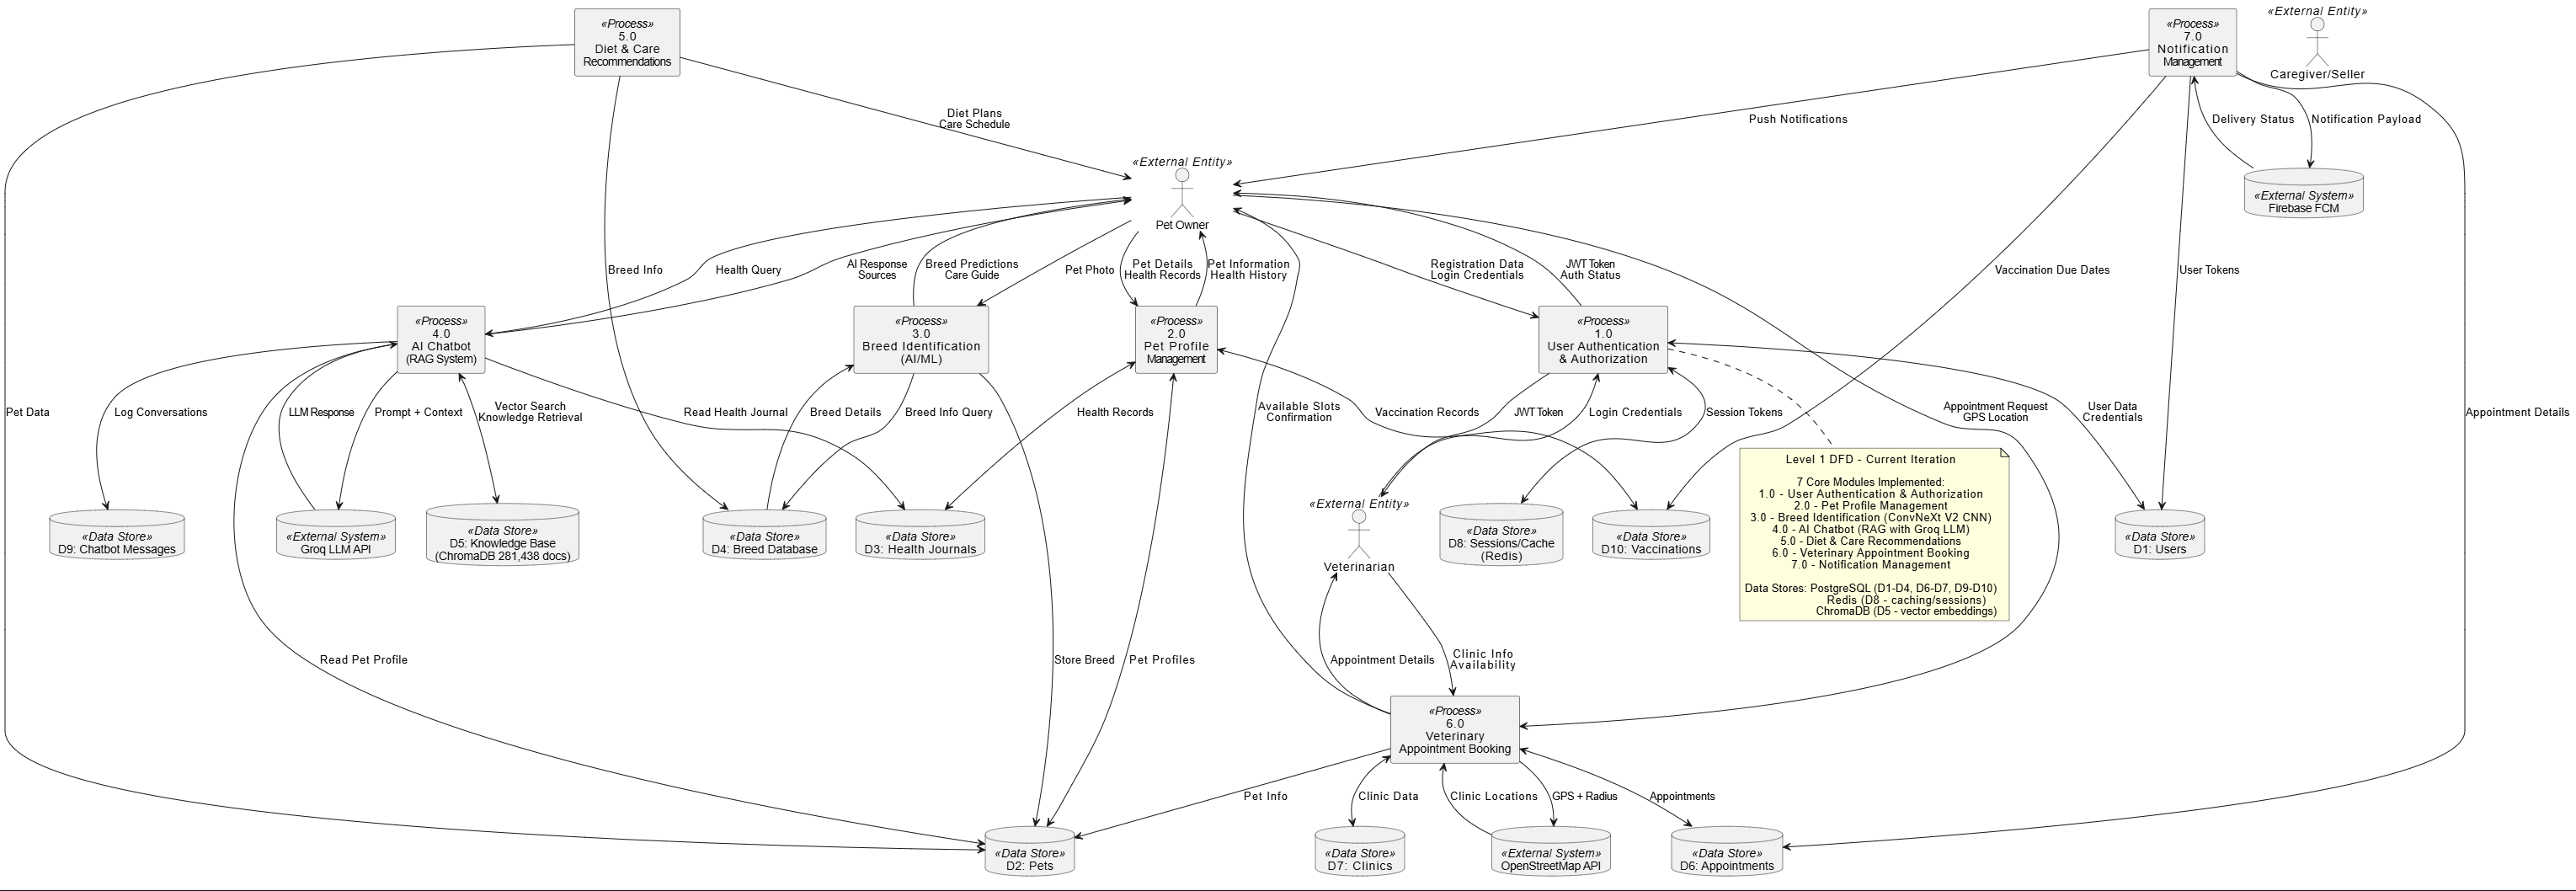
\includegraphics[width=\textwidth]{ThesisFigs/dfd_level1.png}
    \caption{DFD Level 1: Main system processes with data stores (D1-D10)}
    \label{fig:dfd_level1}
\end{figure}

The Level 1 diagram decomposes the system into seven main processes: User Authentication \& Authorization, Pet Profile Management, Breed Identification (AI/ML), AI Chatbot (RAG System), Diet \& Care Recommendations, Veterinary Appointment Booking, and Notification Management. Data stores include PostgreSQL tables (D1-D4, D6-D7, D9-D10), Redis cache (D8), and ChromaDB vector database (D5) with 281,438 veterinary documents.

\subsubsection{Level 2: Detailed Sub-Processes}

\textbf{User Authentication \& Authorization}

\begin{figure}[H]
    \centering
    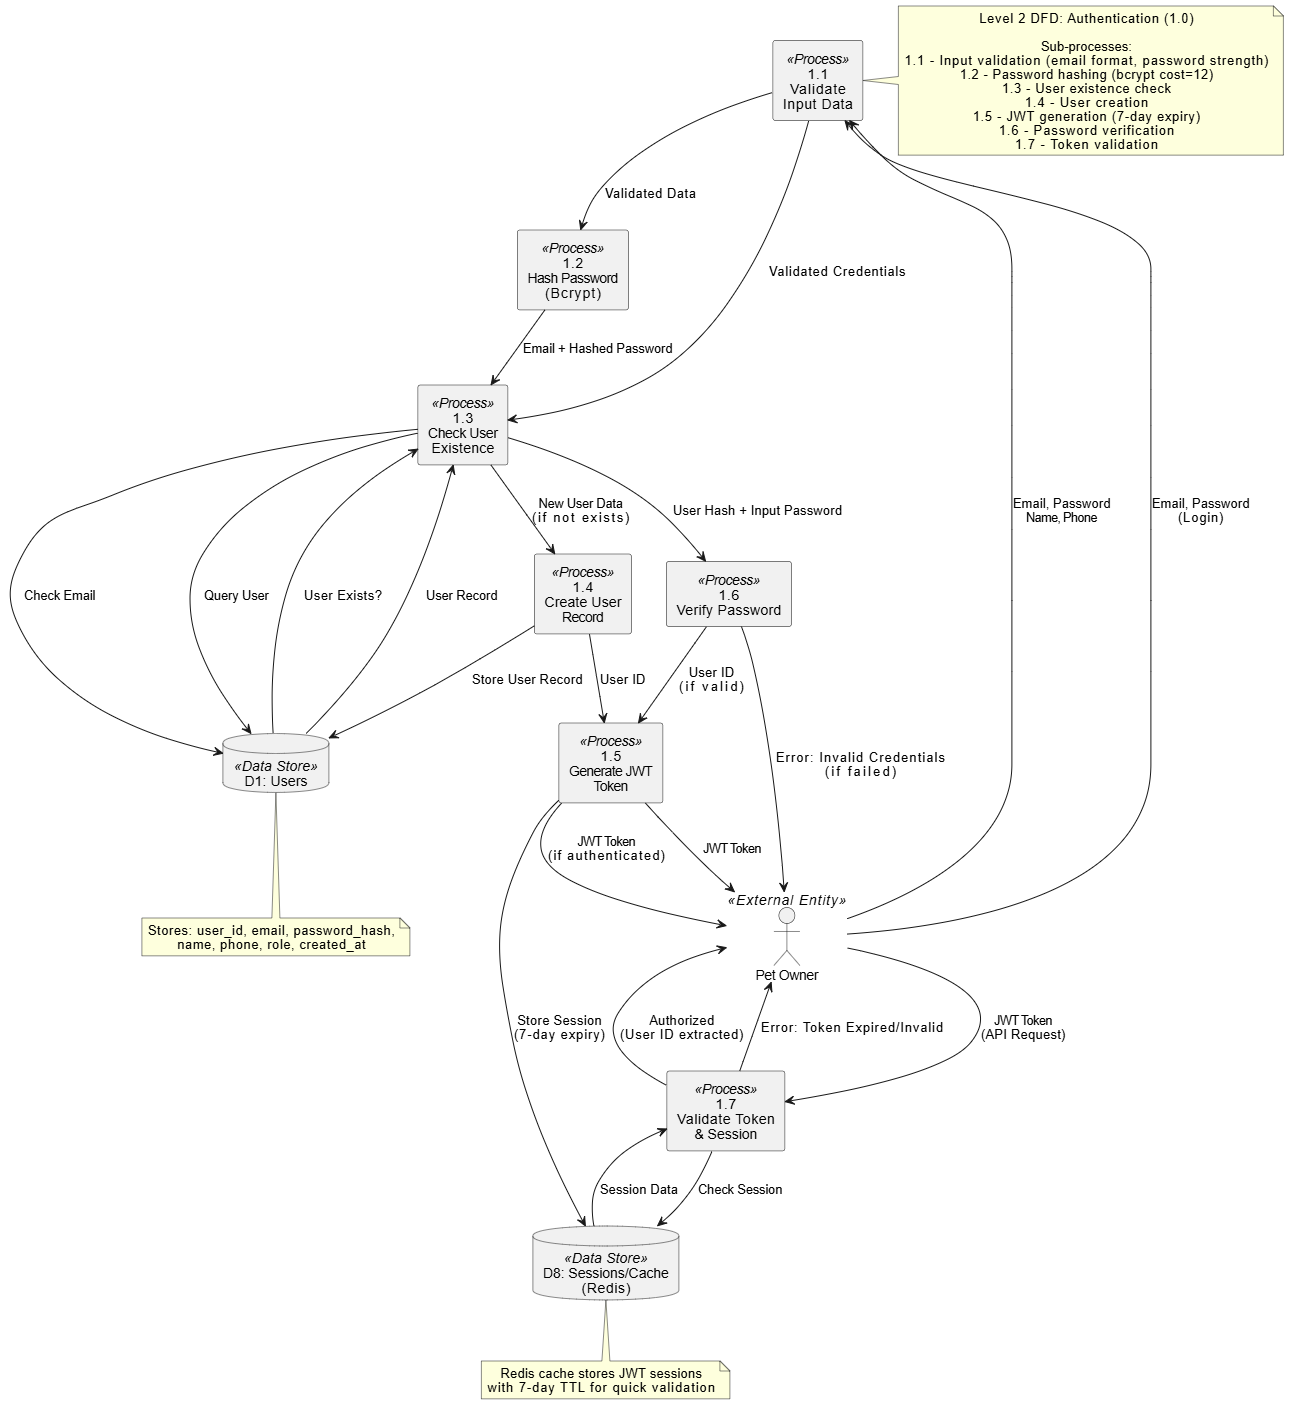
\includegraphics[width=\textwidth]{ThesisFigs/dfd_level2_auth.png}
    \caption{DFD Level 2: User Authentication \& Authorization sub-processes}
    \label{fig:dfd_level2_auth}
\end{figure}

Seven sub-processes handle authentication: input validation, password hashing (bcrypt cost=12), user existence checking, user creation, JWT generation (7-day expiry), password verification, and token validation. Data flows through D1 (Users) and D8 (Redis Sessions).

\textbf{Pet Profile Management}

\begin{figure}[H]
    \centering
    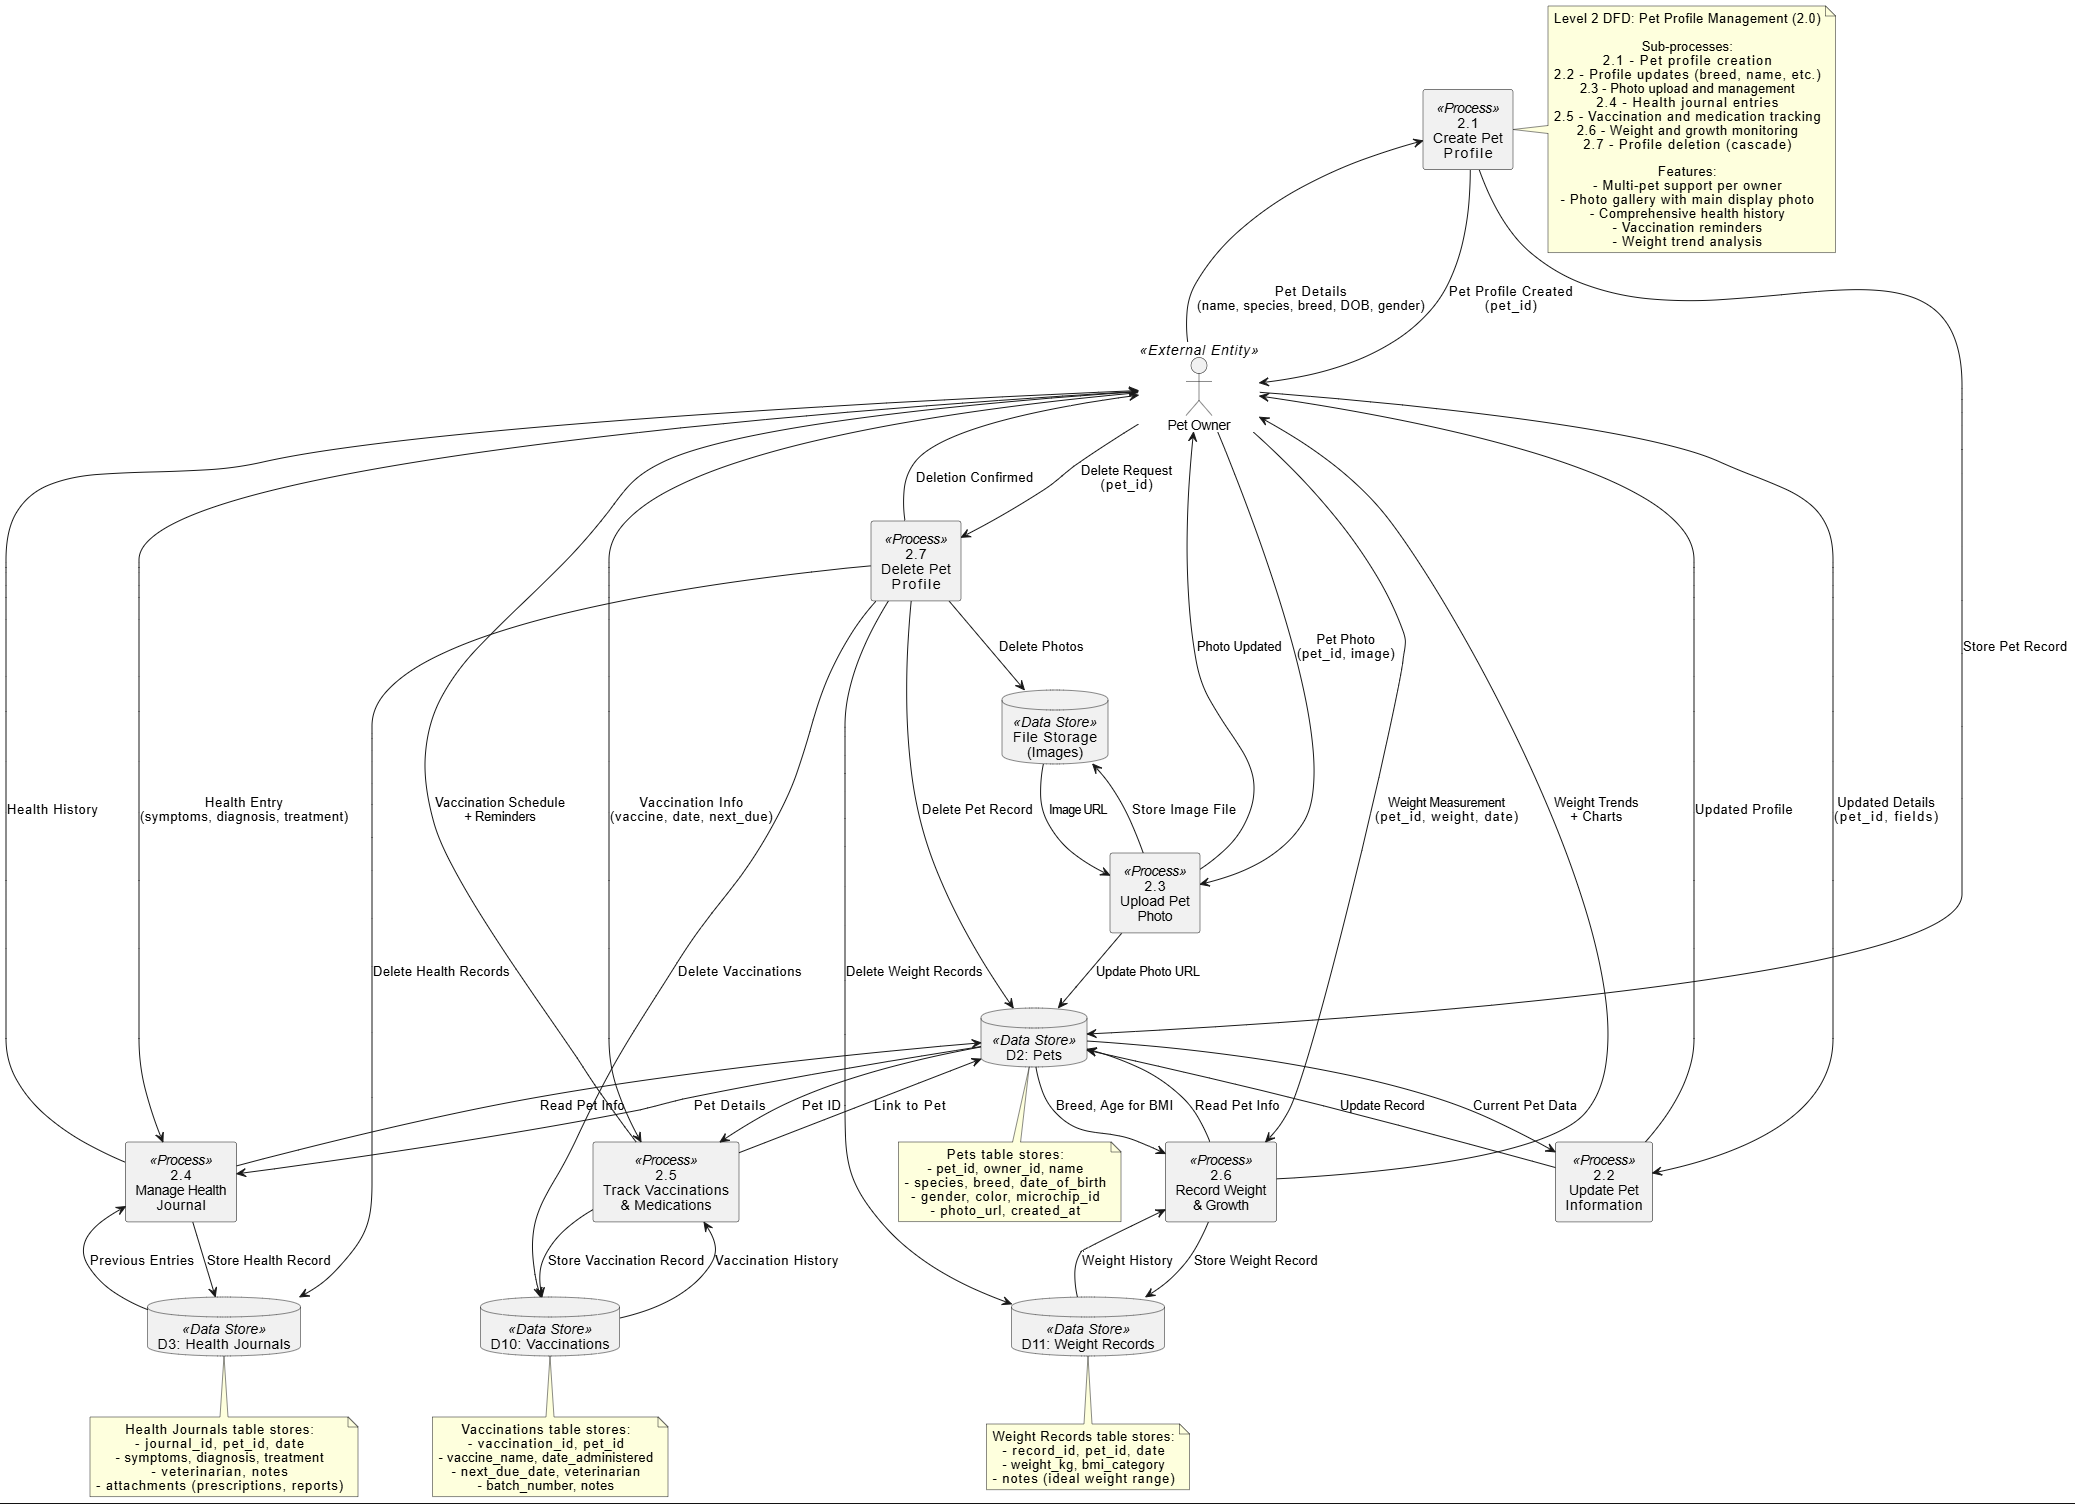
\includegraphics[width=\textwidth]{ThesisFigs/dfd_level2_pet_managment.png}
    \caption{DFD Level 2: Pet Profile Management sub-processes}
    \label{fig:dfd_level2_pet}
\end{figure}

Seven sub-processes manage pet data: create pet profile, update profile, upload photo, manage health journal, track vaccinations/medications, record weight/growth, and delete pet with cascade. Interacts with D2 (Pets), D3 (Health Journals), and D10 (Vaccinations).

\textbf{Breed Identification}

\begin{figure}[H]
    \centering
    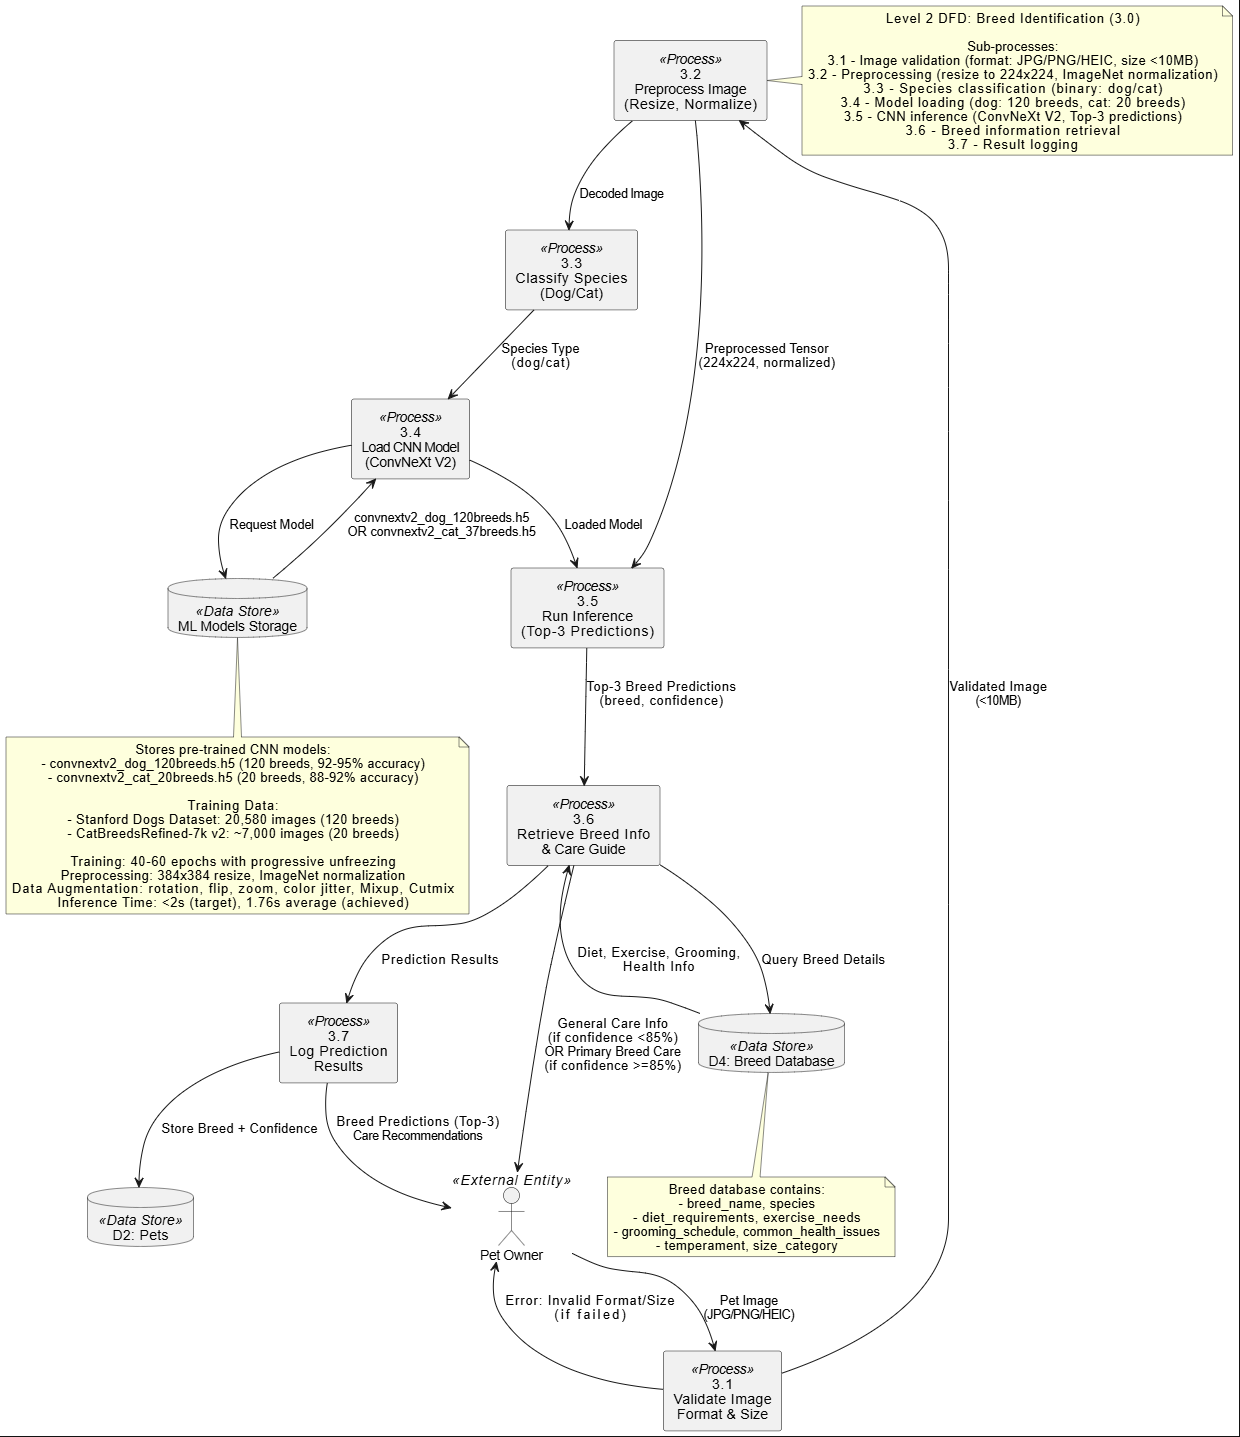
\includegraphics[width=\textwidth]{ThesisFigs/dfd_level2_breed.png}
    \caption{DFD Level 2: Breed Identification sub-processes using ConvNeXt V2 CNN}
    \label{fig:dfd_level2_breed}
\end{figure}

Seven sub-processes handle breed classification: image validation (format/size), preprocessing (384x384 resize, ImageNet normalization), species classification (dog/cat), CNN model loading (120 dog breeds with 92-95\% accuracy, 20 cat breeds with 88-92\% accuracy), inference (Top-3 predictions), breed information retrieval, and result logging. Uses ML Models Storage and D4 (Breed Database).

\textbf{AI Chatbot (RAG Pipeline)}

\begin{figure}[H]
    \centering
    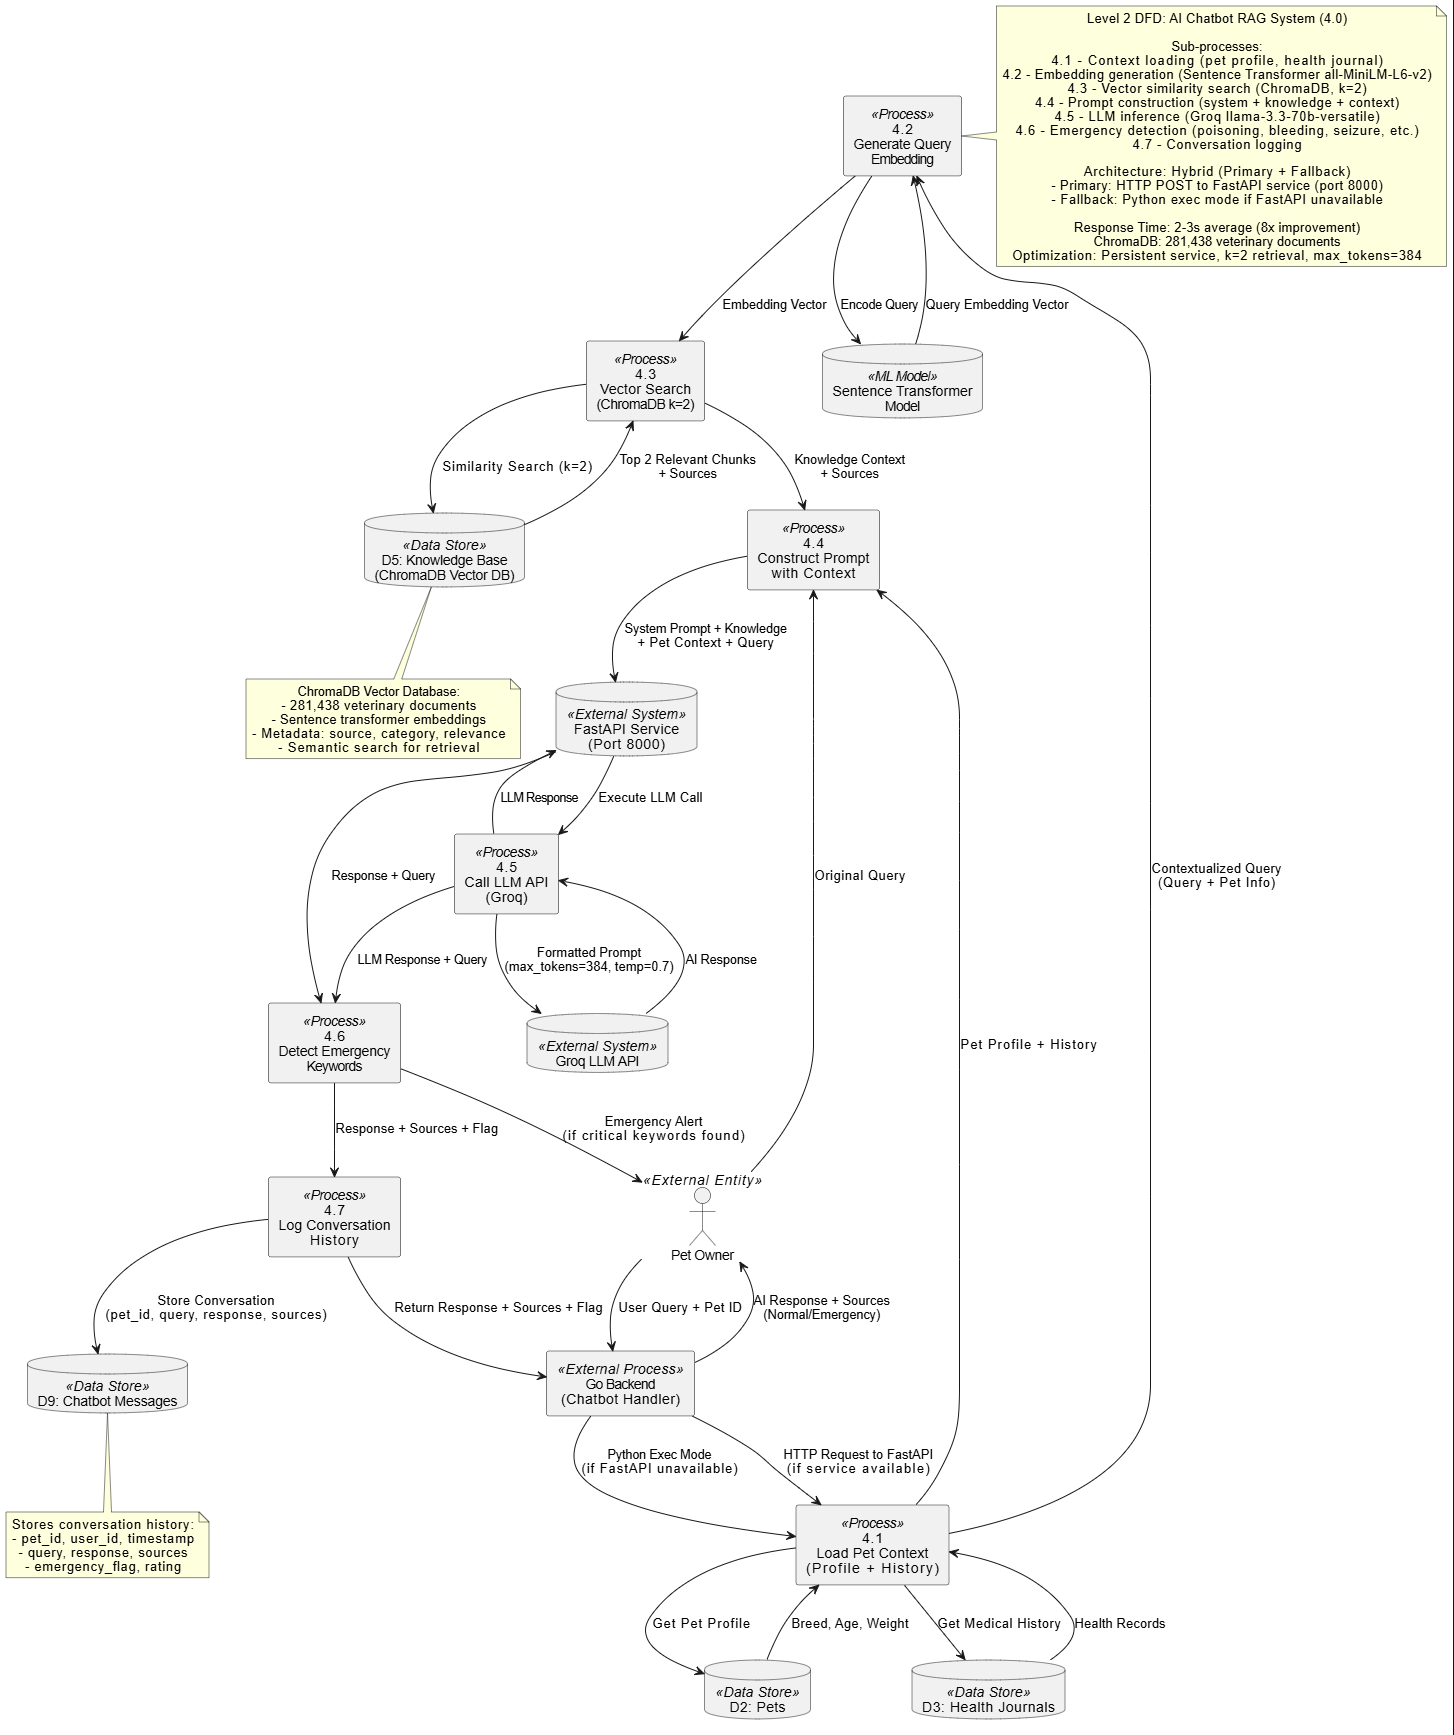
\includegraphics[width=\textwidth]{ThesisFigs/dfd_level2_ai.png}
    \caption{DFD Level 2: AI Chatbot (RAG Pipeline) sub-processes}
    \label{fig:dfd_level2_ai}
\end{figure}

Seven sub-processes power the RAG system: load pet context from profile/health records, generate query embedding (all-MiniLM-L6-v2), perform vector search in ChromaDB (k=2 retrieval), construct contextualized prompt, call Groq LLM API (llama-3.3-70b-versatile), detect emergency keywords, and log conversation. FastAPI service runs on port 8000 with persistent RAG pipeline achieving 2-3s response time. Hybrid architecture supports HTTP mode (primary) and exec mode (fallback).

\textbf{Diet \& Care Recommendations}

\begin{figure}[H]
    \centering
    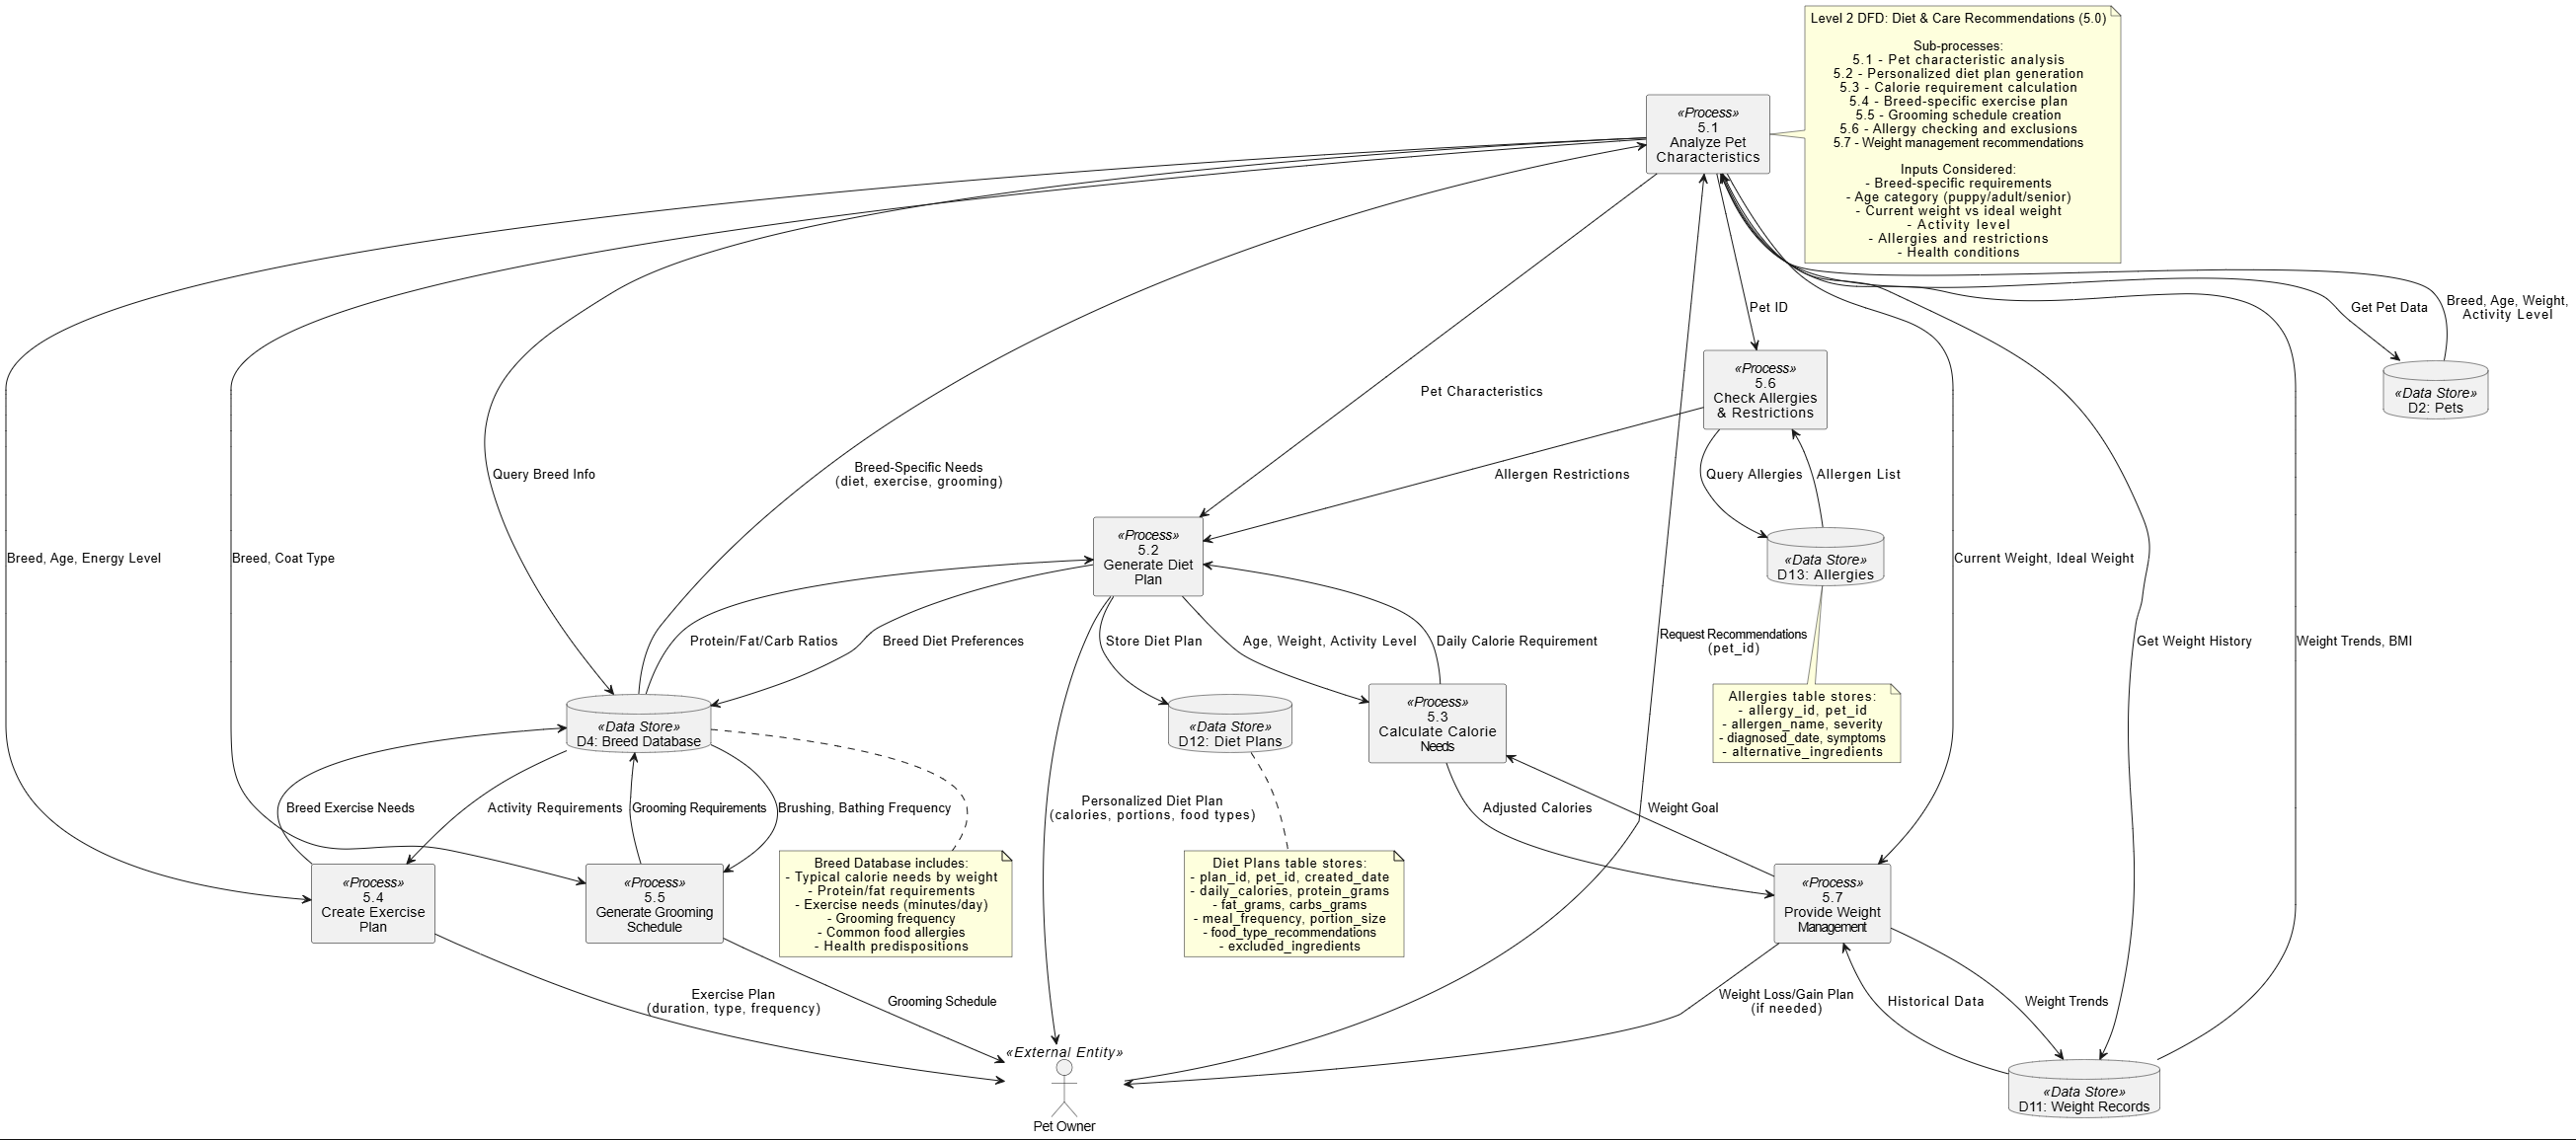
\includegraphics[width=\textwidth]{ThesisFigs/dfd_level2_diet.png}
    \caption{DFD Level 2: Diet \& Care Recommendations sub-processes}
    \label{fig:dfd_level2_diet}
\end{figure}

Seven sub-processes generate personalized care plans: analyze pet characteristics (breed, age, weight, activity), generate breed-specific diet plan, calculate daily calorie needs, create exercise plan, generate grooming schedule, check allergies/restrictions, and provide weight management guidance. Uses D2 (Pets) and D4 (Breed Database).

\textbf{Veterinary Appointment Booking}

\begin{figure}[H]
    \centering
    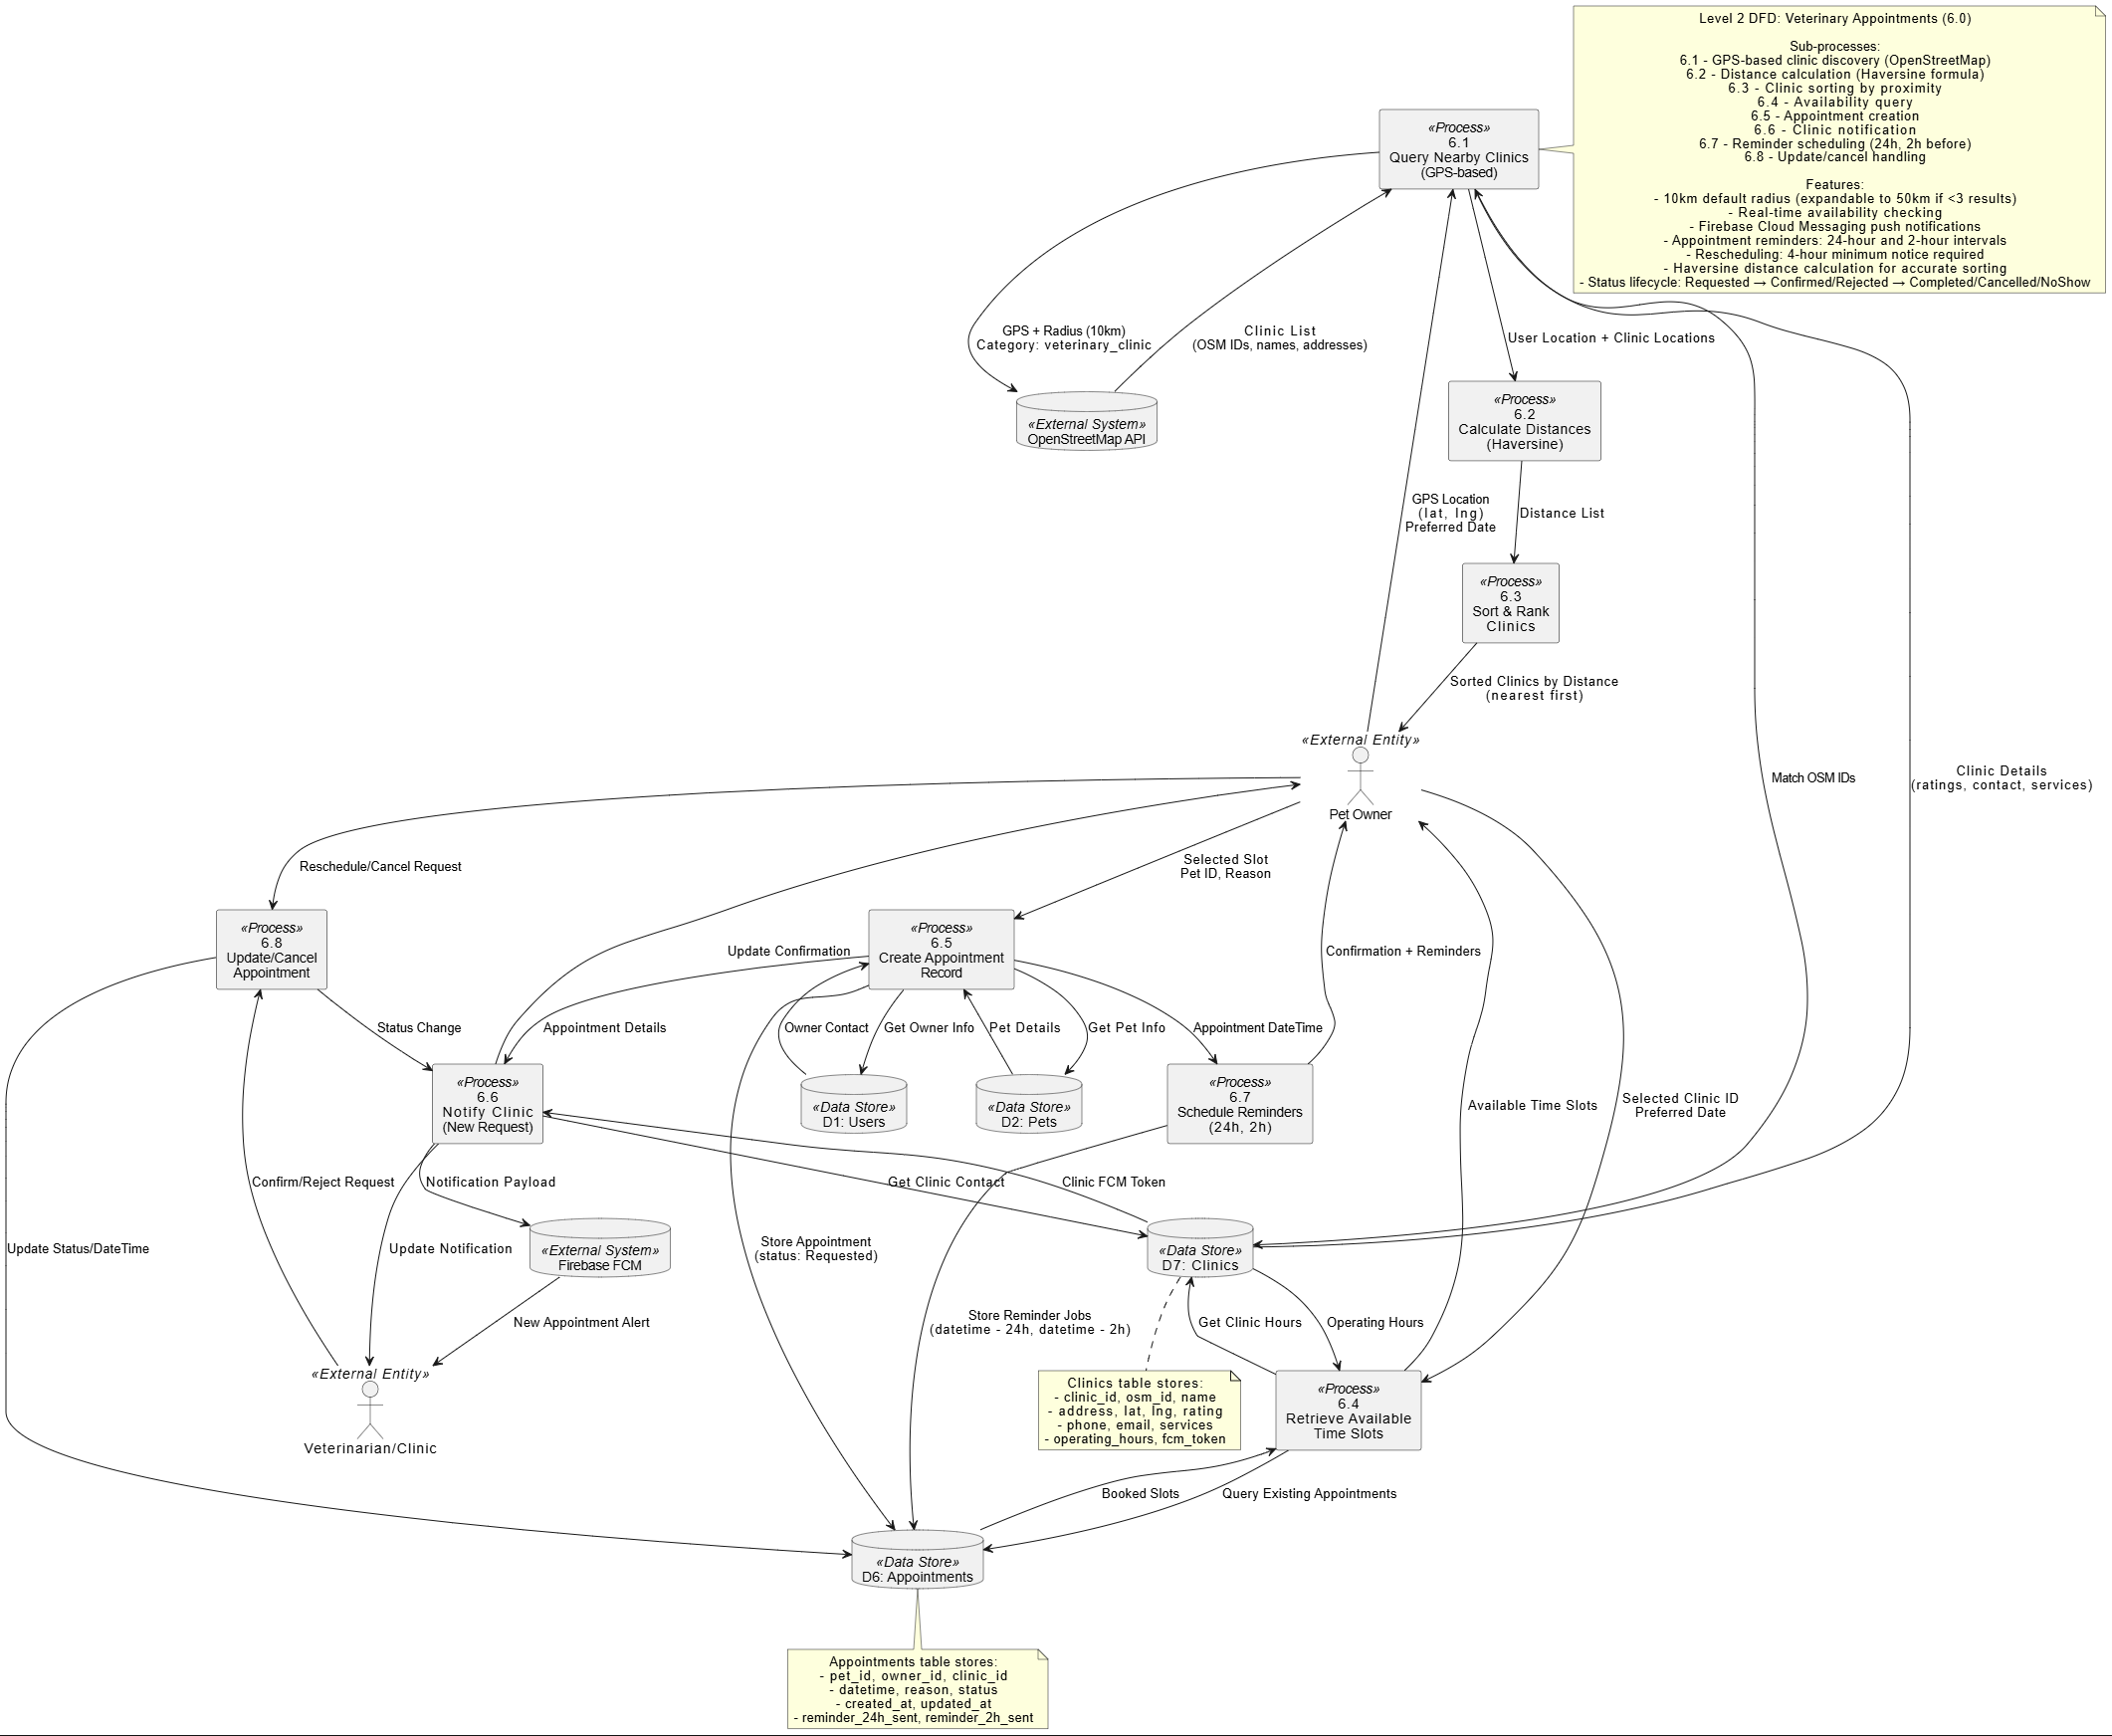
\includegraphics[width=\textwidth]{ThesisFigs/dfd_level2_vet.png}
    \caption{DFD Level 2: Veterinary Appointment Booking sub-processes}
    \label{fig:dfd_level2_vet}
\end{figure}

Eight sub-processes manage appointments: GPS-based clinic discovery (OpenStreetMap 10km radius), Haversine distance calculation, clinic sorting by proximity, availability query, appointment creation, clinic notification via Firebase FCM, reminder scheduling (24-hour and 2-hour intervals), and update/cancel handling (4-hour minimum notice). Interacts with D6 (Appointments), D7 (Clinics), and external APIs.

\textbf{Notification Management}

\begin{figure}[H]
    \centering
    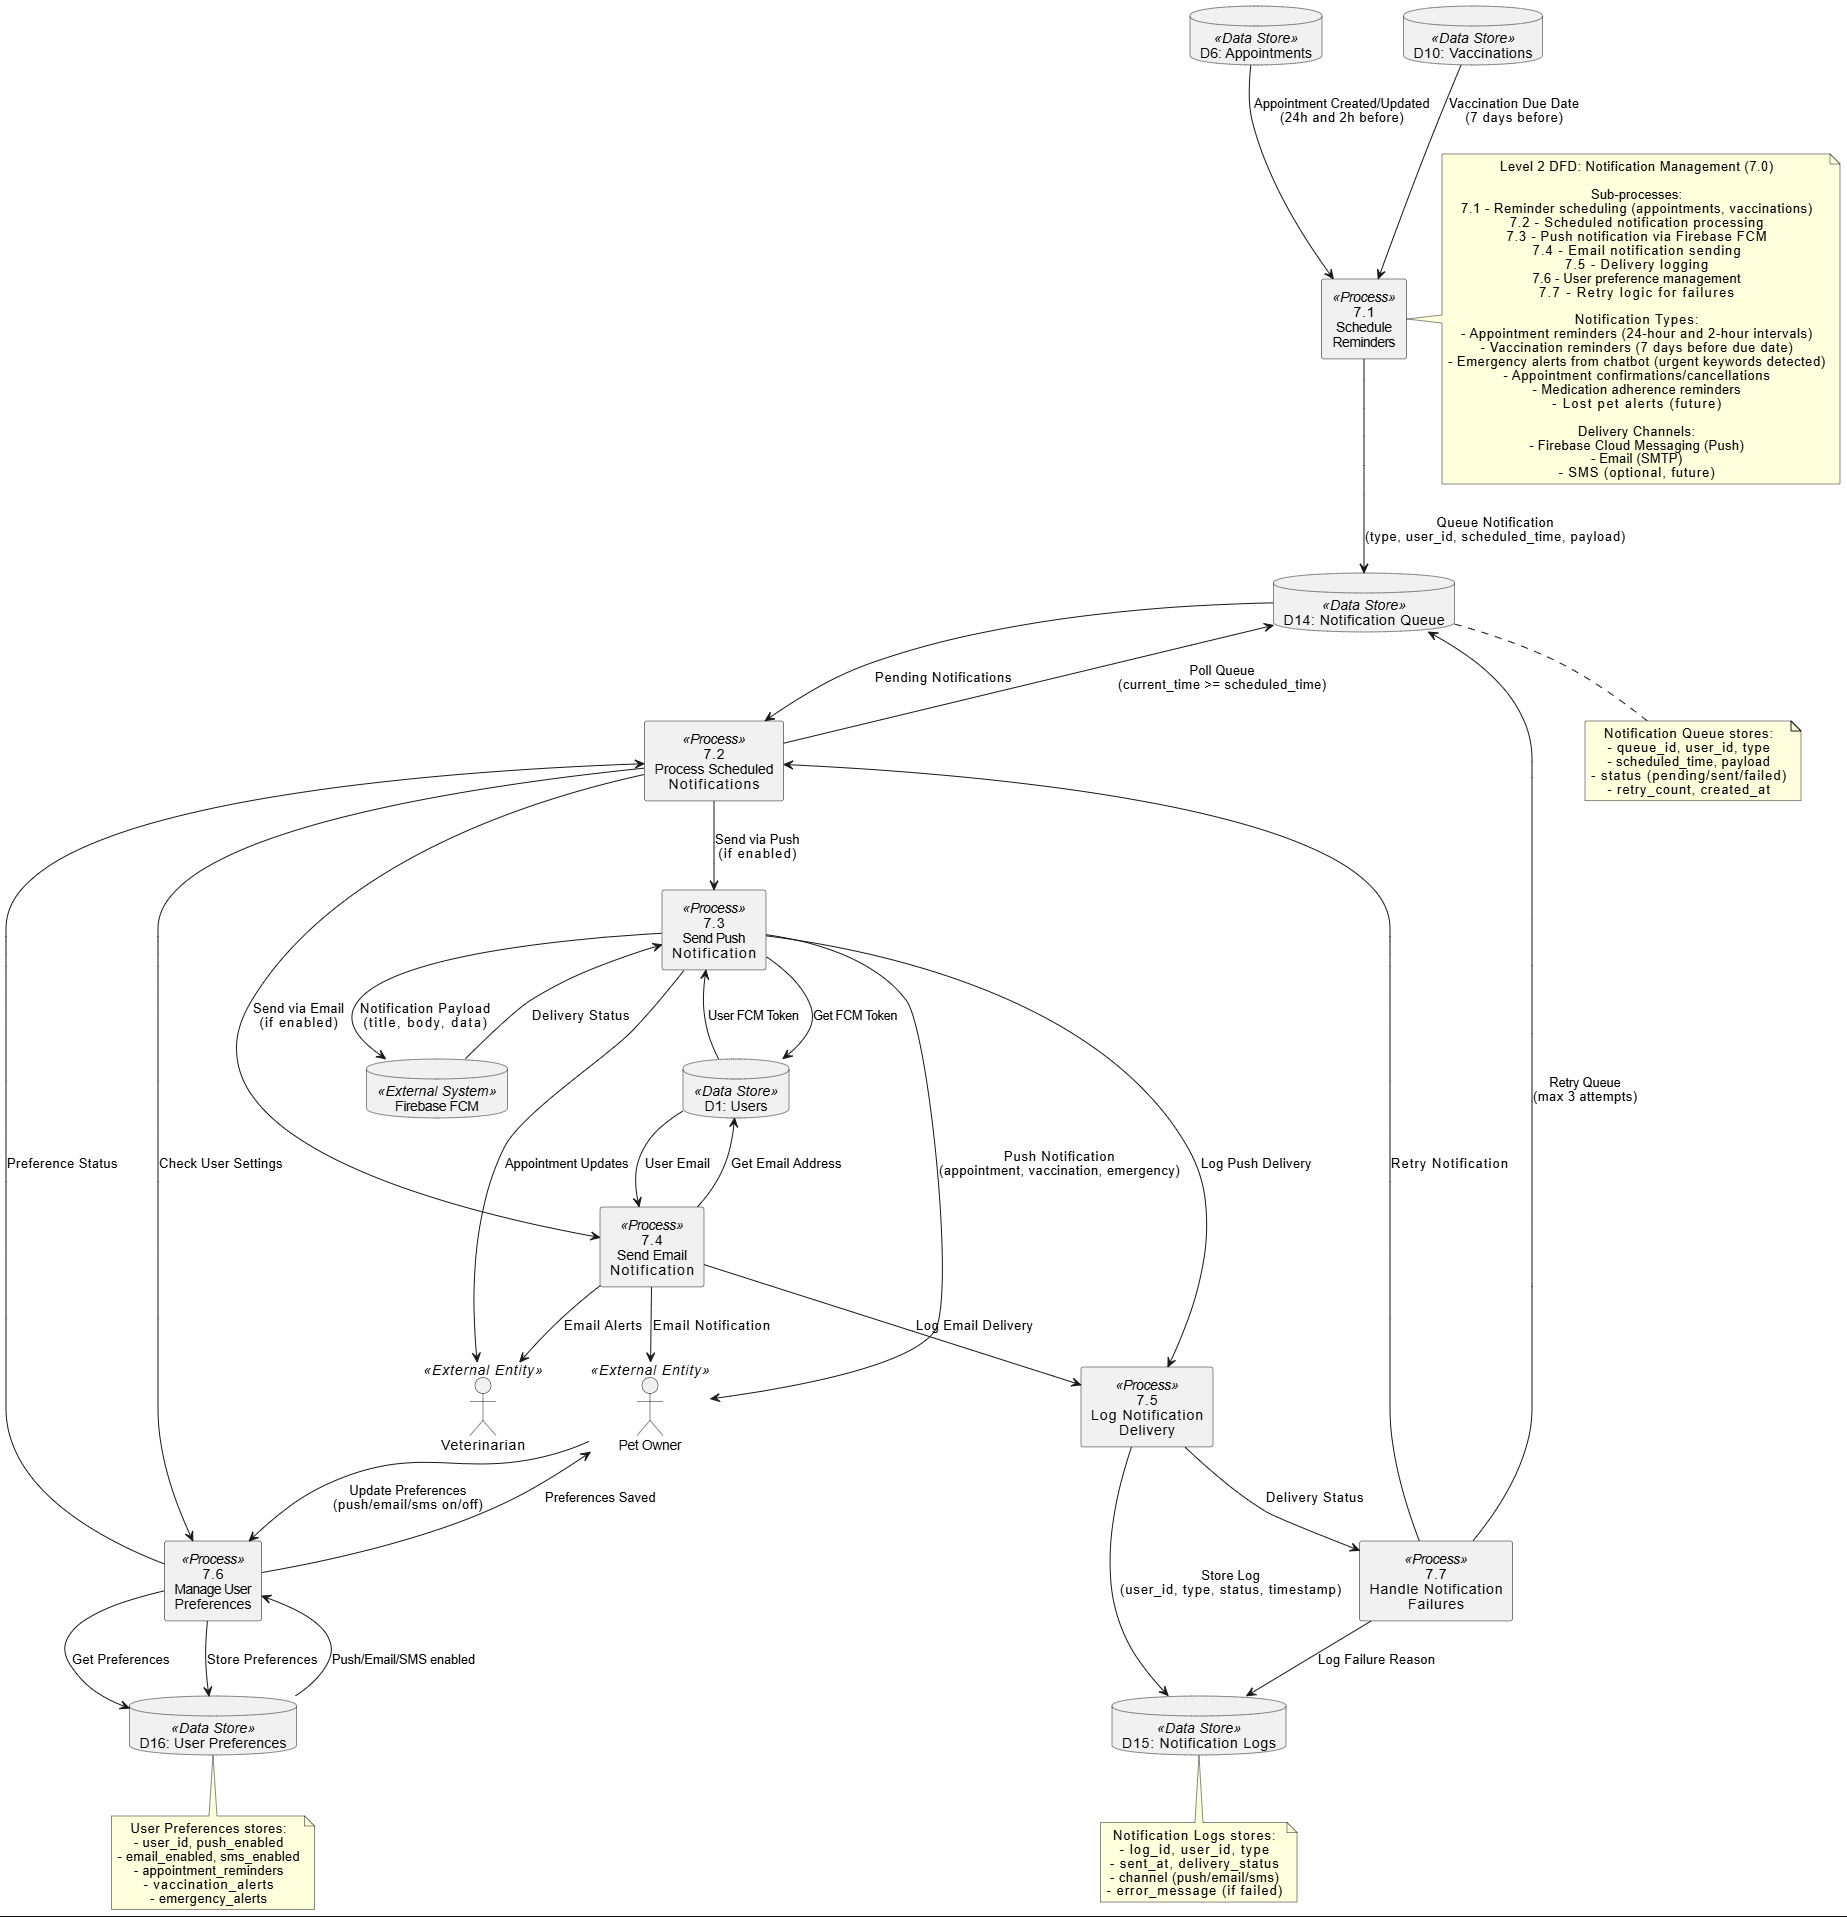
\includegraphics[width=\textwidth]{ThesisFigs/dfd_level2_notification.png}
    \caption{DFD Level 2: Notification Management sub-processes}
    \label{fig:dfd_level2_notification}
\end{figure}

Seven sub-processes handle notifications: schedule reminders (appointments, vaccinations 7 days before due date), process scheduled notifications, send push notifications via Firebase FCM, send email notifications, log delivery status, manage user preferences, and handle notification failures with retry logic.

\subsection{Database Schema Overview}

\textbf{User Management:} users (authentication), user\_profiles (extended info), user\_roles (RBAC), user\_sessions (active sessions).

\textbf{Pet Management:} pets (profiles with breed/medical history), health\_journals (event timeline), vaccinations (records/due dates), medications (schedules), vet\_visits (history), pet\_photos (gallery).

\textbf{Marketplace:} products (listings), product\_photos (up to 10/product), orders (status tracking), order\_items (line items), reviews (ratings), shopping\_carts (session-based).

\textbf{Community:} posts (content), comments (threaded), lost\_pets (GPS alerts), adoptions (listings), events (RSVP tracking), sightings (lost pet reports).

\textbf{Service Providers:} veterinarians (clinic profiles), caregivers (profiles), appointments (vet bookings), caregiver\_bookings (services), service\_tracking (GPS data).

\textbf{Payment:} transactions (all payments), crypto\_wallets (addresses), digital\_wallets (credit balances), invoices (receipts).

\textbf{AI/ML:} breed\_identifications (CNN results), chatbot\_conversations (history), chatbot\_messages (timestamped messages).

\subsection{Data Storage Strategies}

\textbf{PostgreSQL:} Primary store with JSONB metadata, indexes on user\_id/pet\_id/timestamp, foreign key constraints, and partitioning for large tables.

\textbf{Redis Caching:} Session tokens (7-day TTL), pet profiles (30-min TTL), API responses (5-min TTL), GPS tracking (2-min TTL), rate limiting counters (1-min sliding window).

\textbf{ChromaDB:} 281,438 veterinary document embeddings (384-dimensional, all-MiniLM-L6-v2), cosine similarity for k=2 retrieval, metadata filters for source tracking.

\section{Domain Model}

The domain model represents core business entities across five domains: Core (User/Pet), Marketplace, Community, Services, and Payment/AI.

\subsection{Core Domain Model}

\begin{figure}[H]
    \centering
    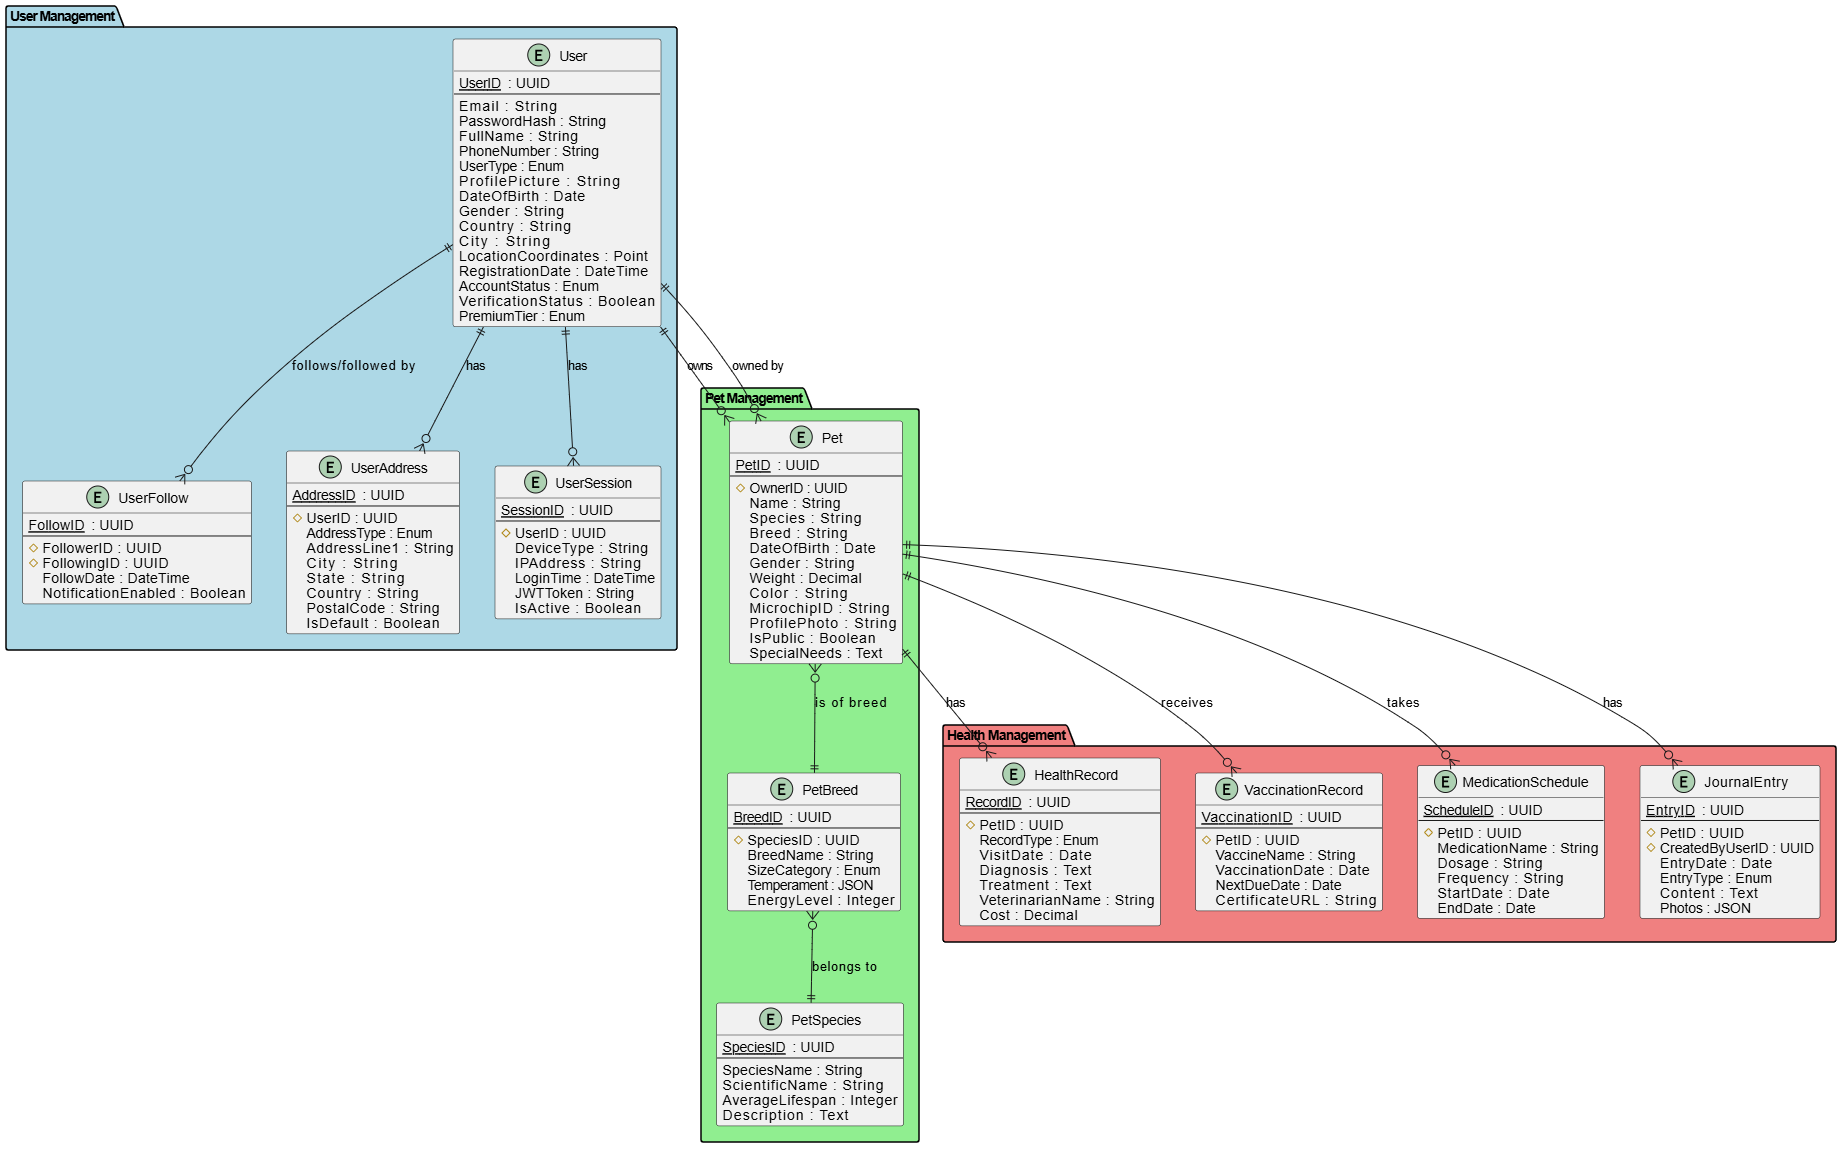
\includegraphics[width=1.0\textwidth]{ThesisFigs/domain_model_core.png}
    \caption{Core Domain Model - User and Pet Entities}
    \label{fig:domain_core}
\end{figure}

User entity with PetOwner/Veterinarian/Caregiver specializations, Pet entity with breed/health records, and 1-to-many relationships with HealthJournal, Vaccination, and Medication.

\subsection{Marketplace Domain Model}

\begin{figure}[H]
    \centering
    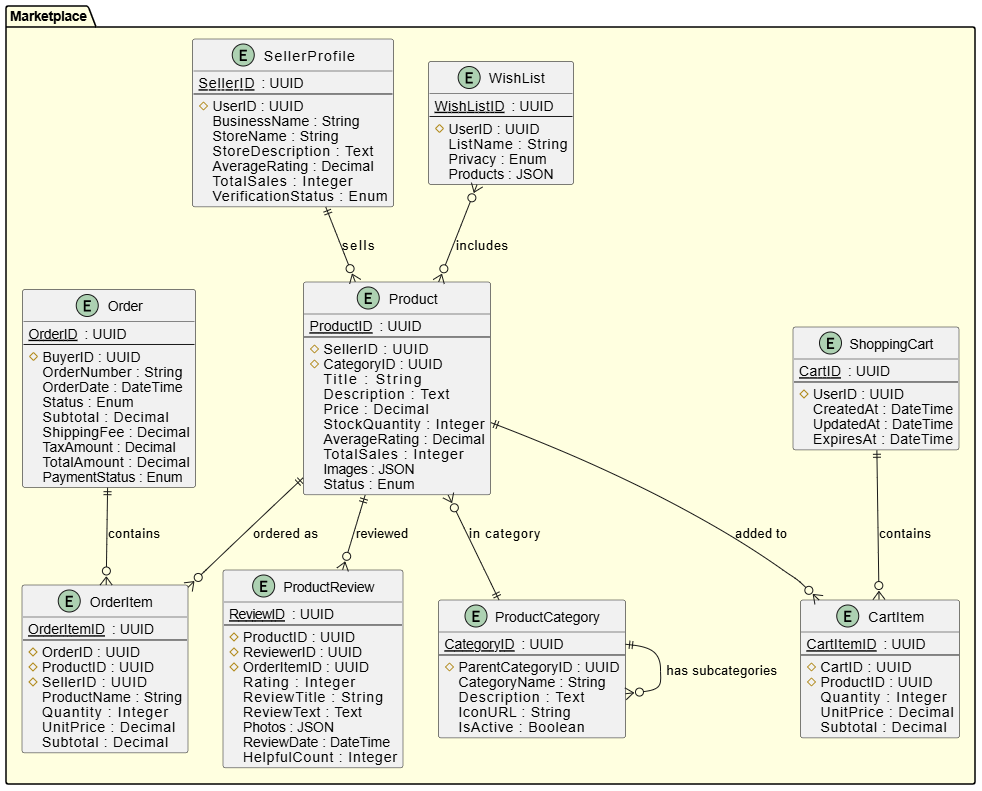
\includegraphics[width=1.0\textwidth]{ThesisFigs/domain_model_marketplace.png}
    \caption{Marketplace Domain Model - E-commerce Entities}
    \label{fig:domain_marketplace}
\end{figure}

Sellers manage Products with ProductPhotos (max 10), PetOwners use ShoppingCart with OrderItems, Orders track fulfillment states, Reviews provide product feedback.

\subsection{Community Domain Model}

\begin{figure}[H]
    \centering
    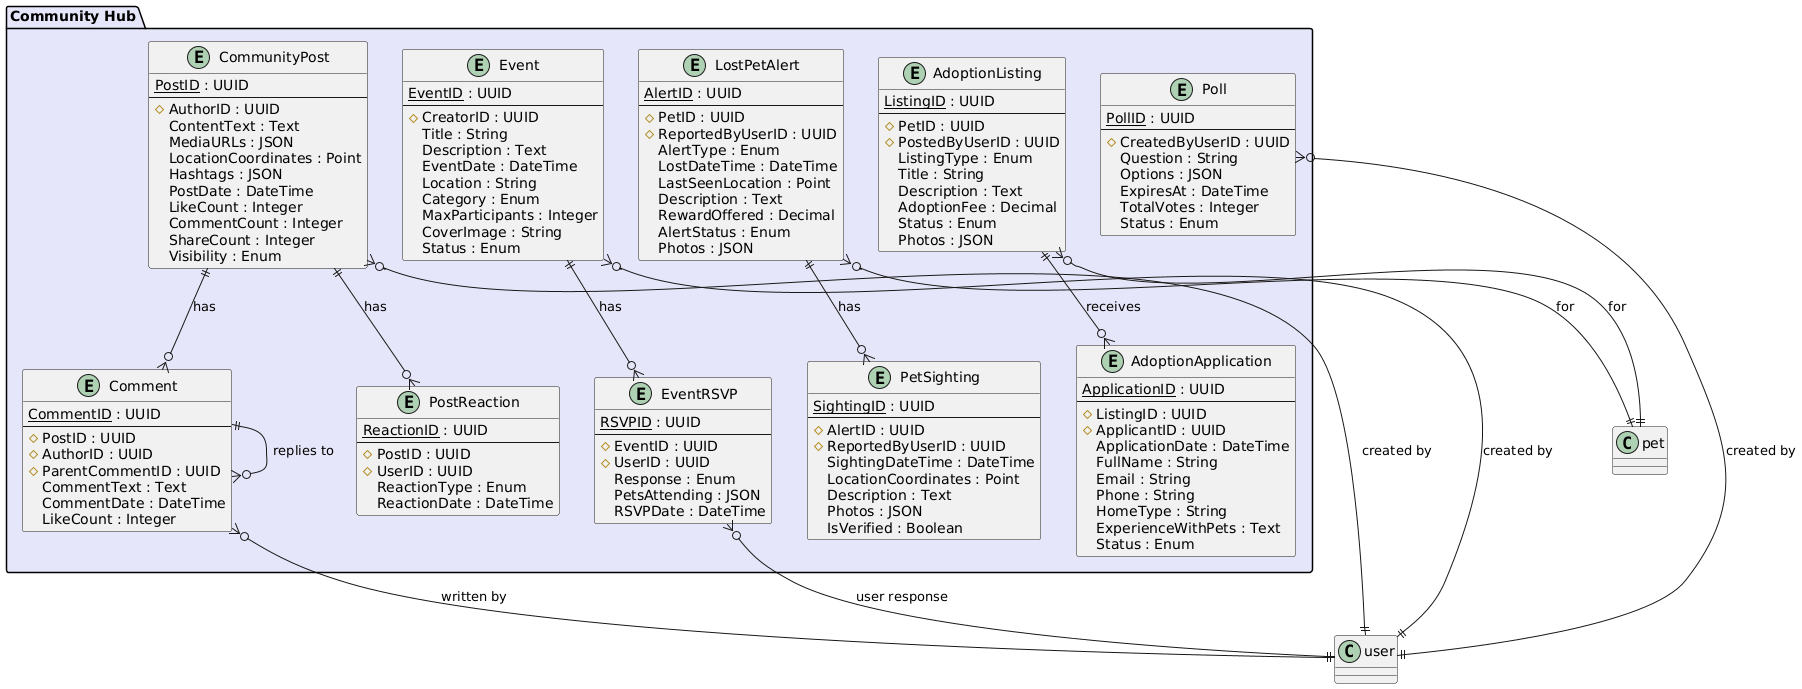
\includegraphics[width=1.0\textwidth]{ThesisFigs/domain_model_community.png}
    \caption{Community Domain Model - Social and Collaboration Entities}
    \label{fig:domain_community}
\end{figure}

Users create Posts with threaded Comments, LostPet alerts with GPS-based Sightings, Adoption listings, Events with RSVP tracking, Groups with many-to-many memberships.

\subsection{Services Domain Model}

\begin{figure}[H]
    \centering
    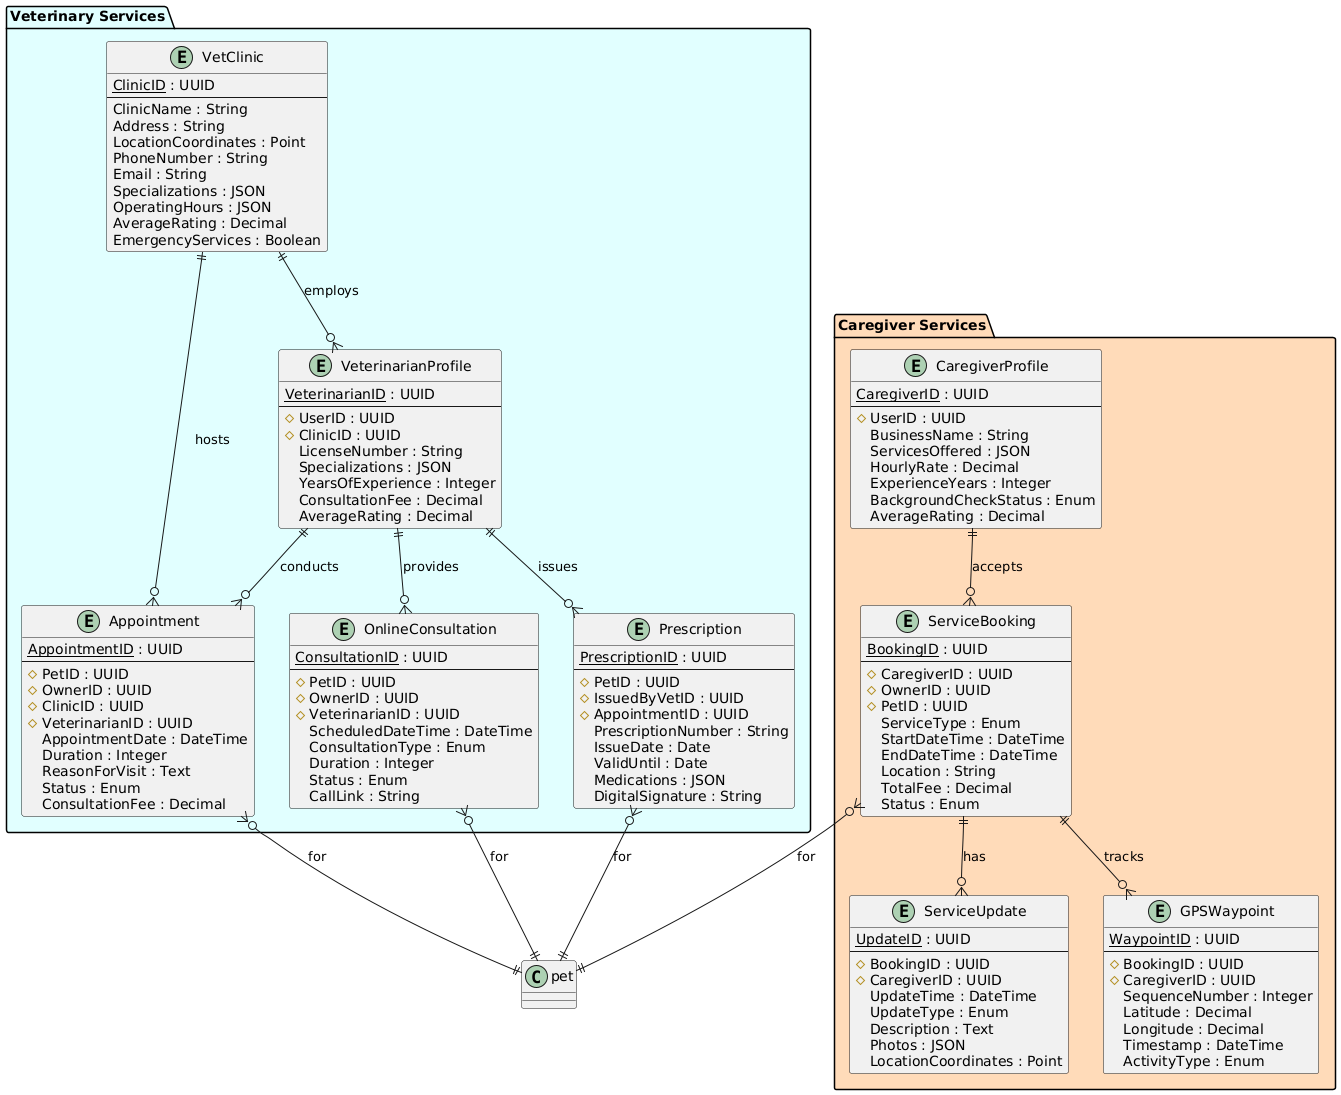
\includegraphics[width=1.0\textwidth]{ThesisFigs/domain_model_services.png}
    \caption{Services Domain Model - Veterinary and Caregiver Entities}
    \label{fig:domain_services}
\end{figure}

VeterinaryClinics employ Veterinarians hosting Appointments with OnlineConsultation and Prescriptions, Caregivers offer CaregiverServices with CaregiverBookings and GPSTracking.

\subsection{Payment and AI Domain Model}

\begin{figure}[H]
    \centering
    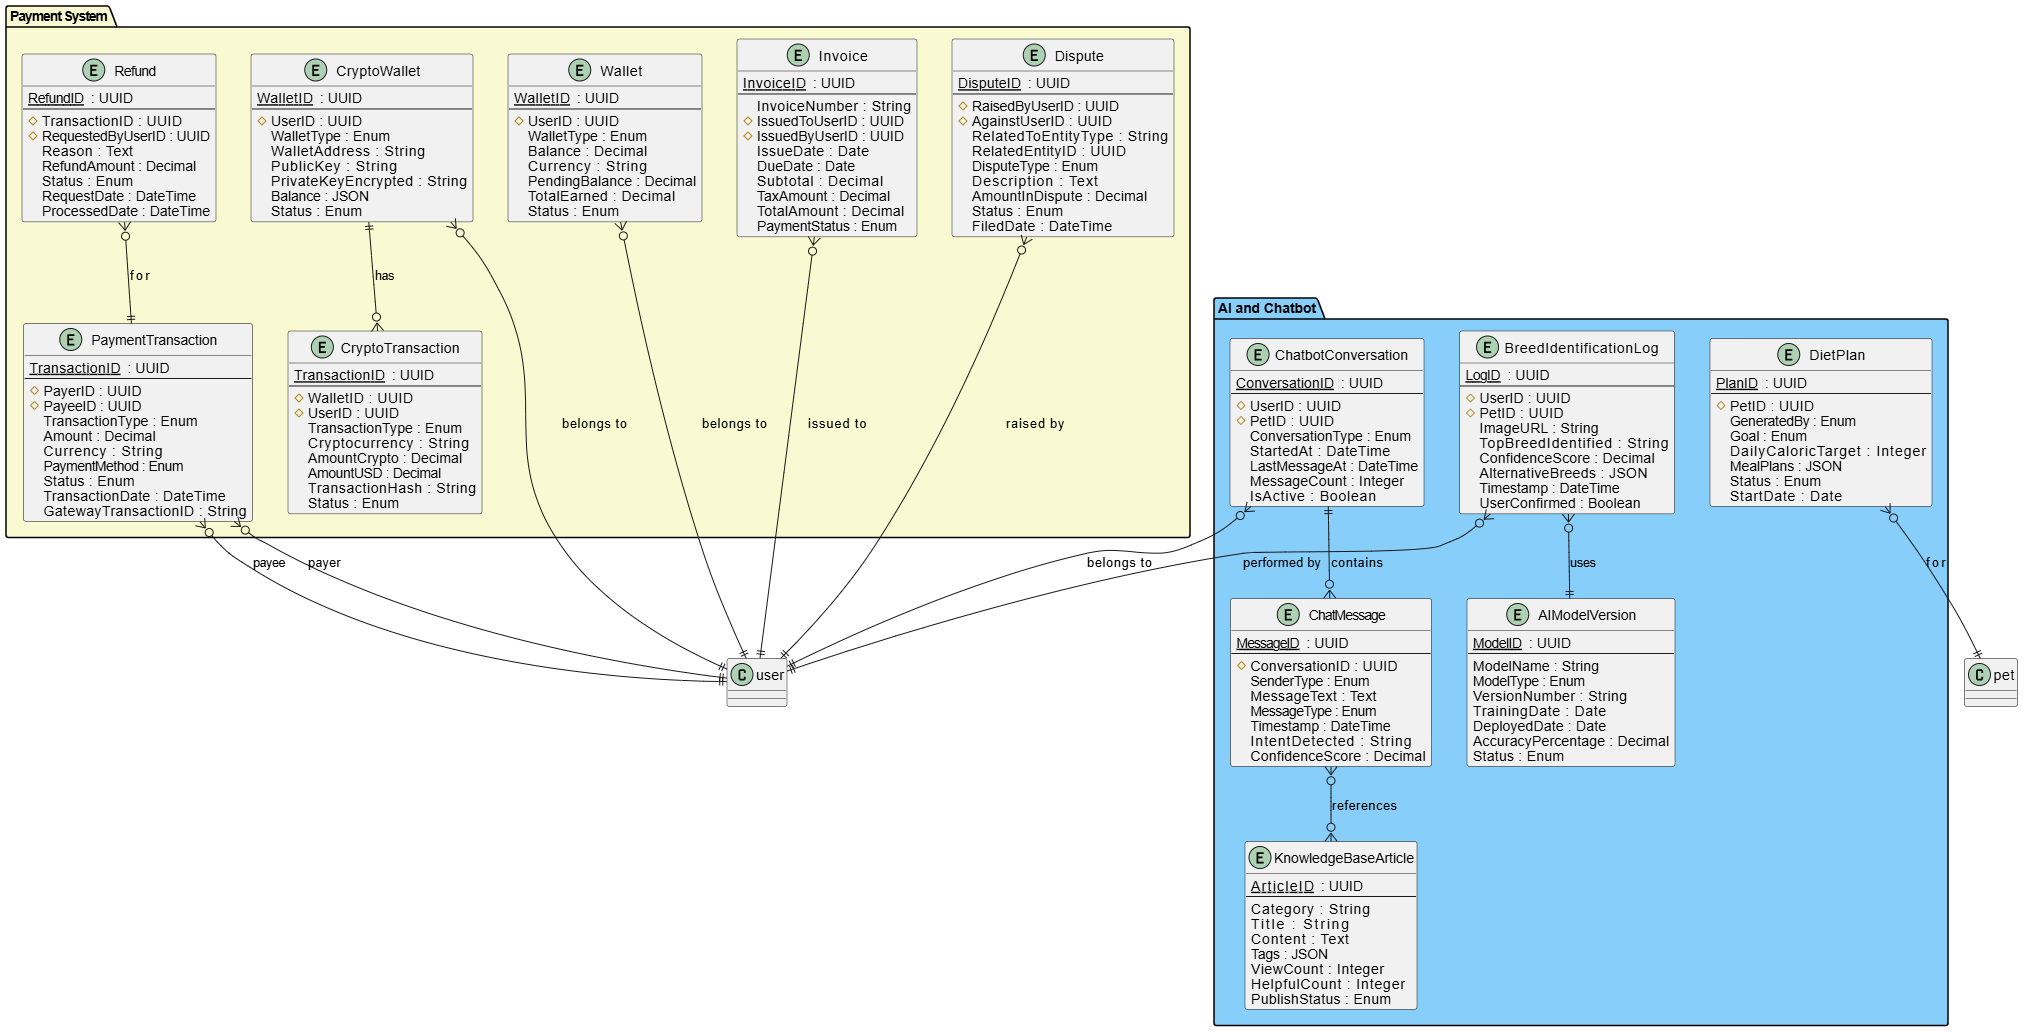
\includegraphics[width=1.0\textwidth]{ThesisFigs/domain_model_payment_ai.png}
    \caption{Payment and AI Domain Model - Transaction and ML Entities}
    \label{fig:domain_payment_ai}
\end{figure}

Transactions support cryptocurrency via CryptoWallet, DigitalWallet credit balances, BreedIdentification stores CNN results with confidence scores, ChatbotConversation maintains RAG message history.

\section{Design Models [Current Iteration]}

This section presents UML diagrams for the current iteration: User Authentication, Pet Breed Identification, AI Chatbot, Diet/Care Recommendations, Veterinary Appointments, Backend Infrastructure, and UI/UX Components.

\subsection{Activity Diagrams}

\subsubsection{User Registration and Authentication}

\begin{figure}[H]
    \centering
    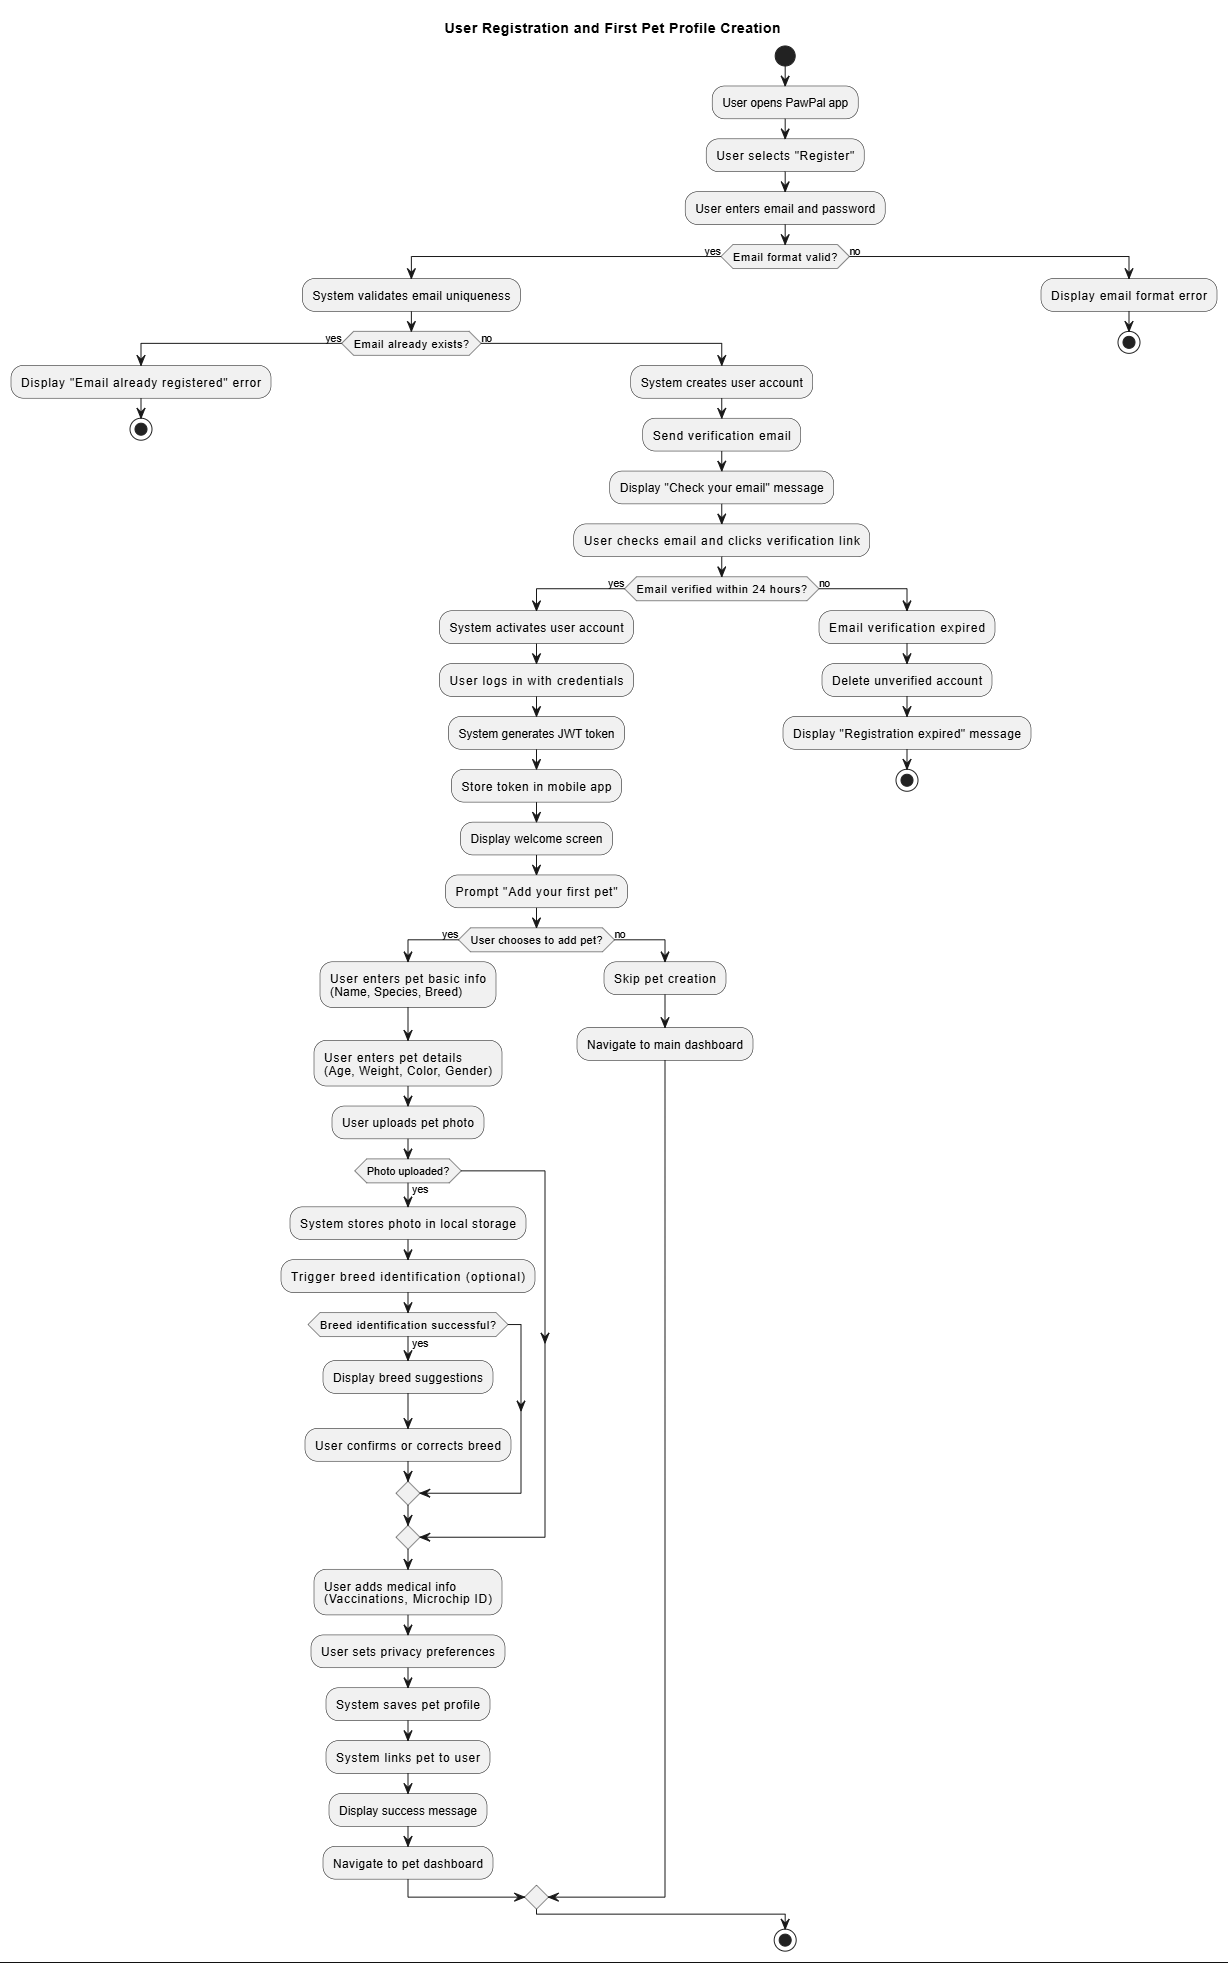
\includegraphics[width=0.9\textwidth]{ThesisFigs/activity_user_registration.png}
    \caption{User Registration and Authentication Activity Diagram}
    \label{fig:activity_user_registration}
\end{figure}

User opens app → enters credentials → system validates email/password → sends verification code → user verifies → system creates account and JWT token → redirects to profile. Decision points: email exists (login redirect), invalid code (retry).

\subsubsection{Pet Breed Identification}

\begin{figure}[H]
    \centering
    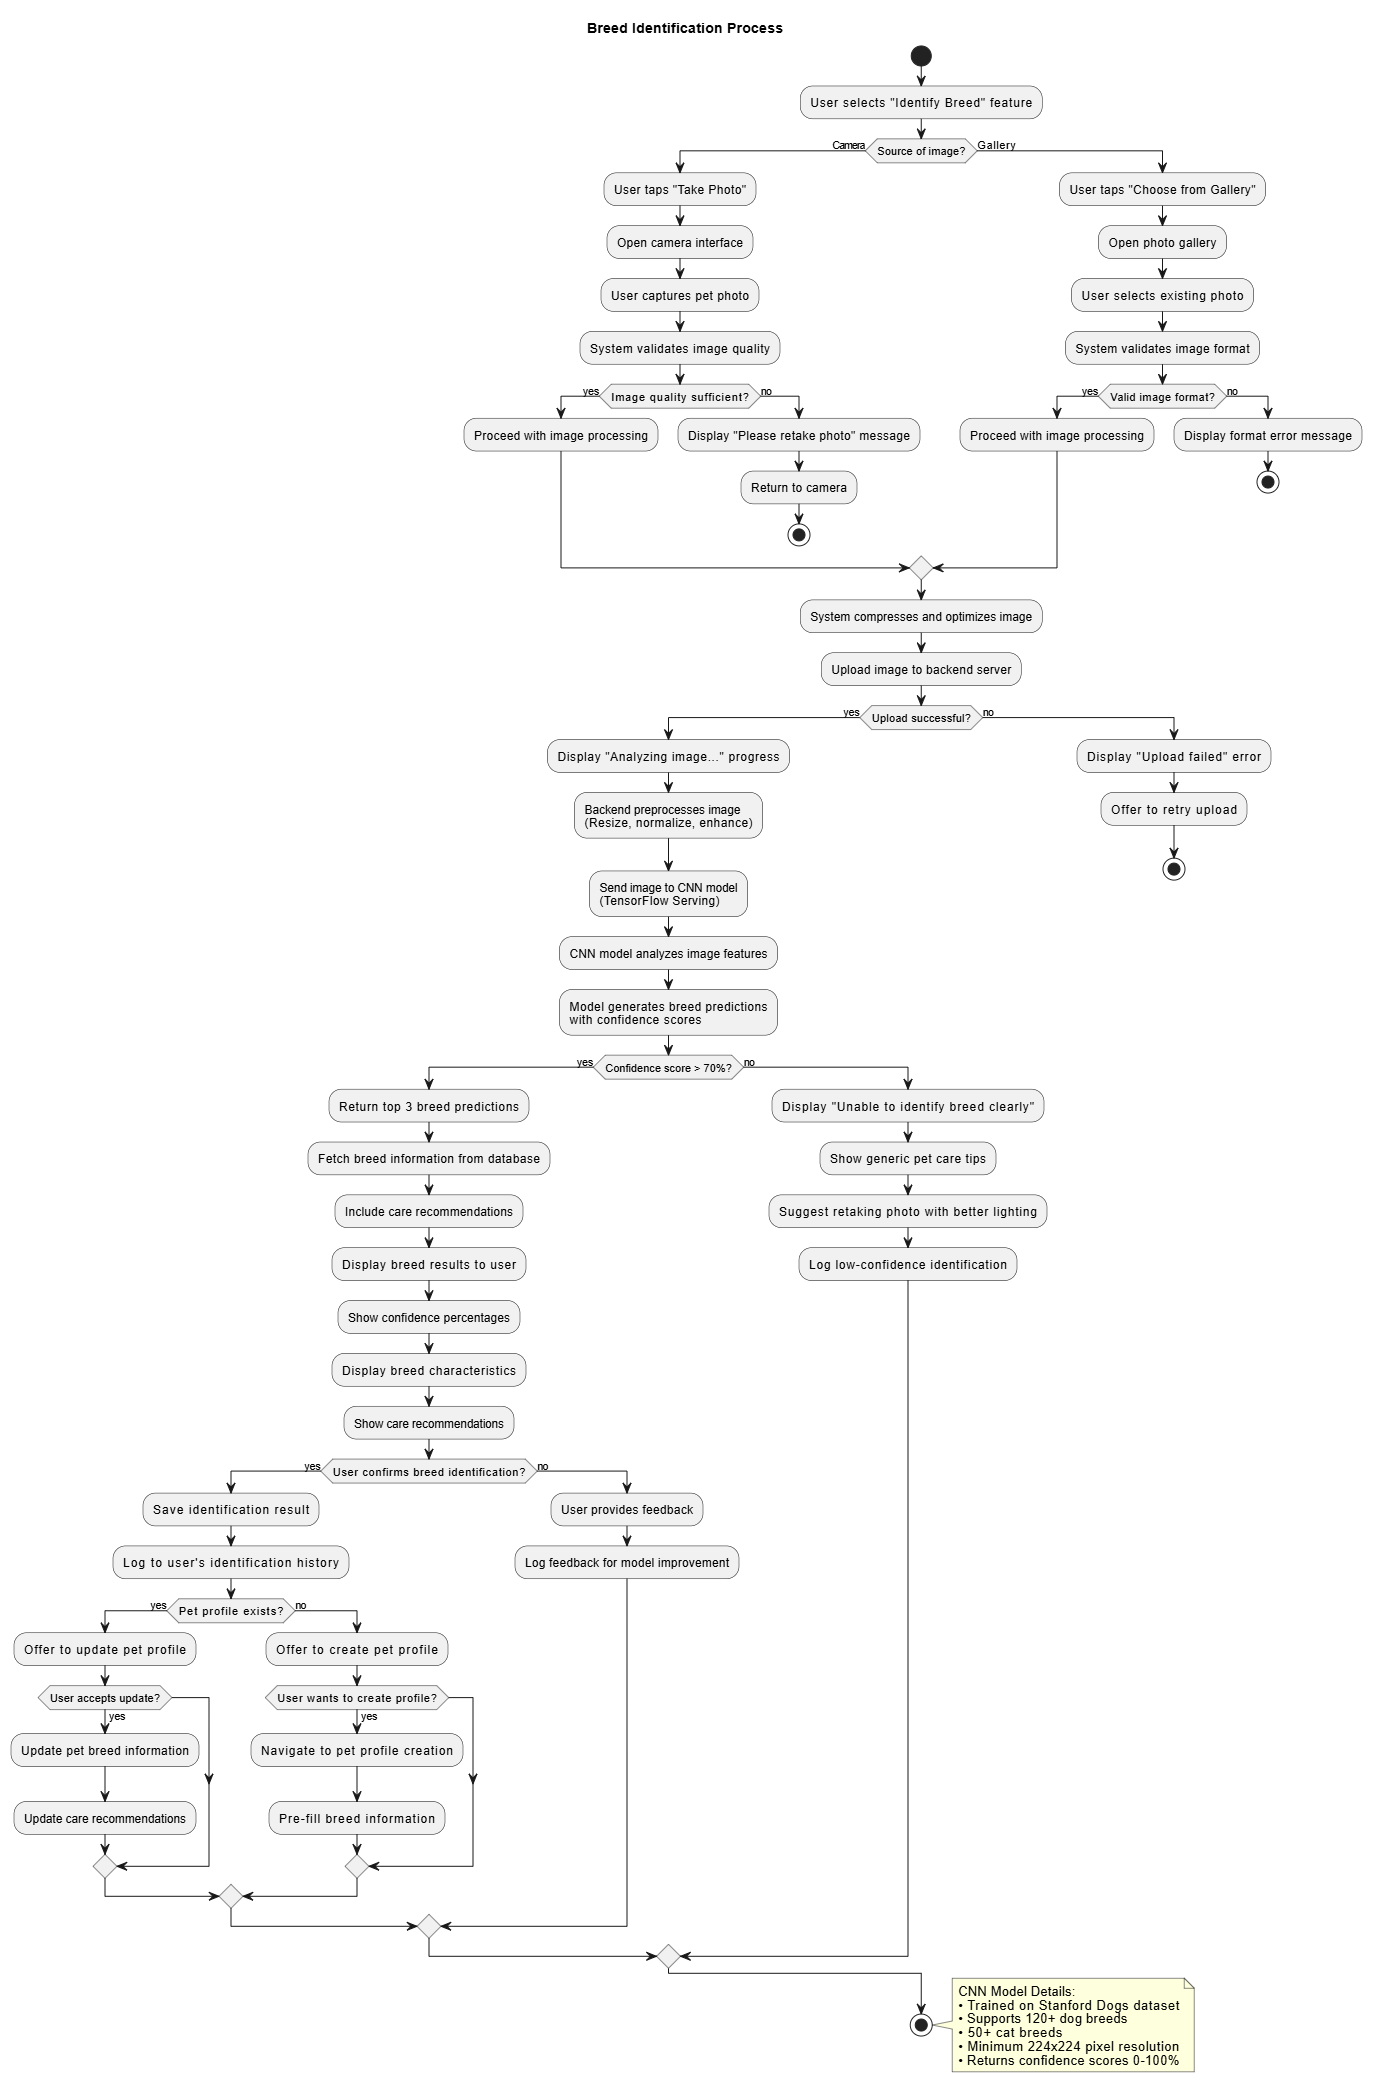
\includegraphics[width=0.9\textwidth]{ThesisFigs/activity_breed_identification.png}
    \caption{Pet Breed Identification Activity Diagram}
    \label{fig:activity_breed_identification}
\end{figure}

User uploads image → system validates → preprocesses (resize/normalize) → sends to CNN → receives top 3 predictions → displays primary if confidence >85\% → user confirms → retrieves care recommendations → updates profile.

\subsubsection{Chatbot RAG Query Processing}

\begin{figure}[H]
    \centering
    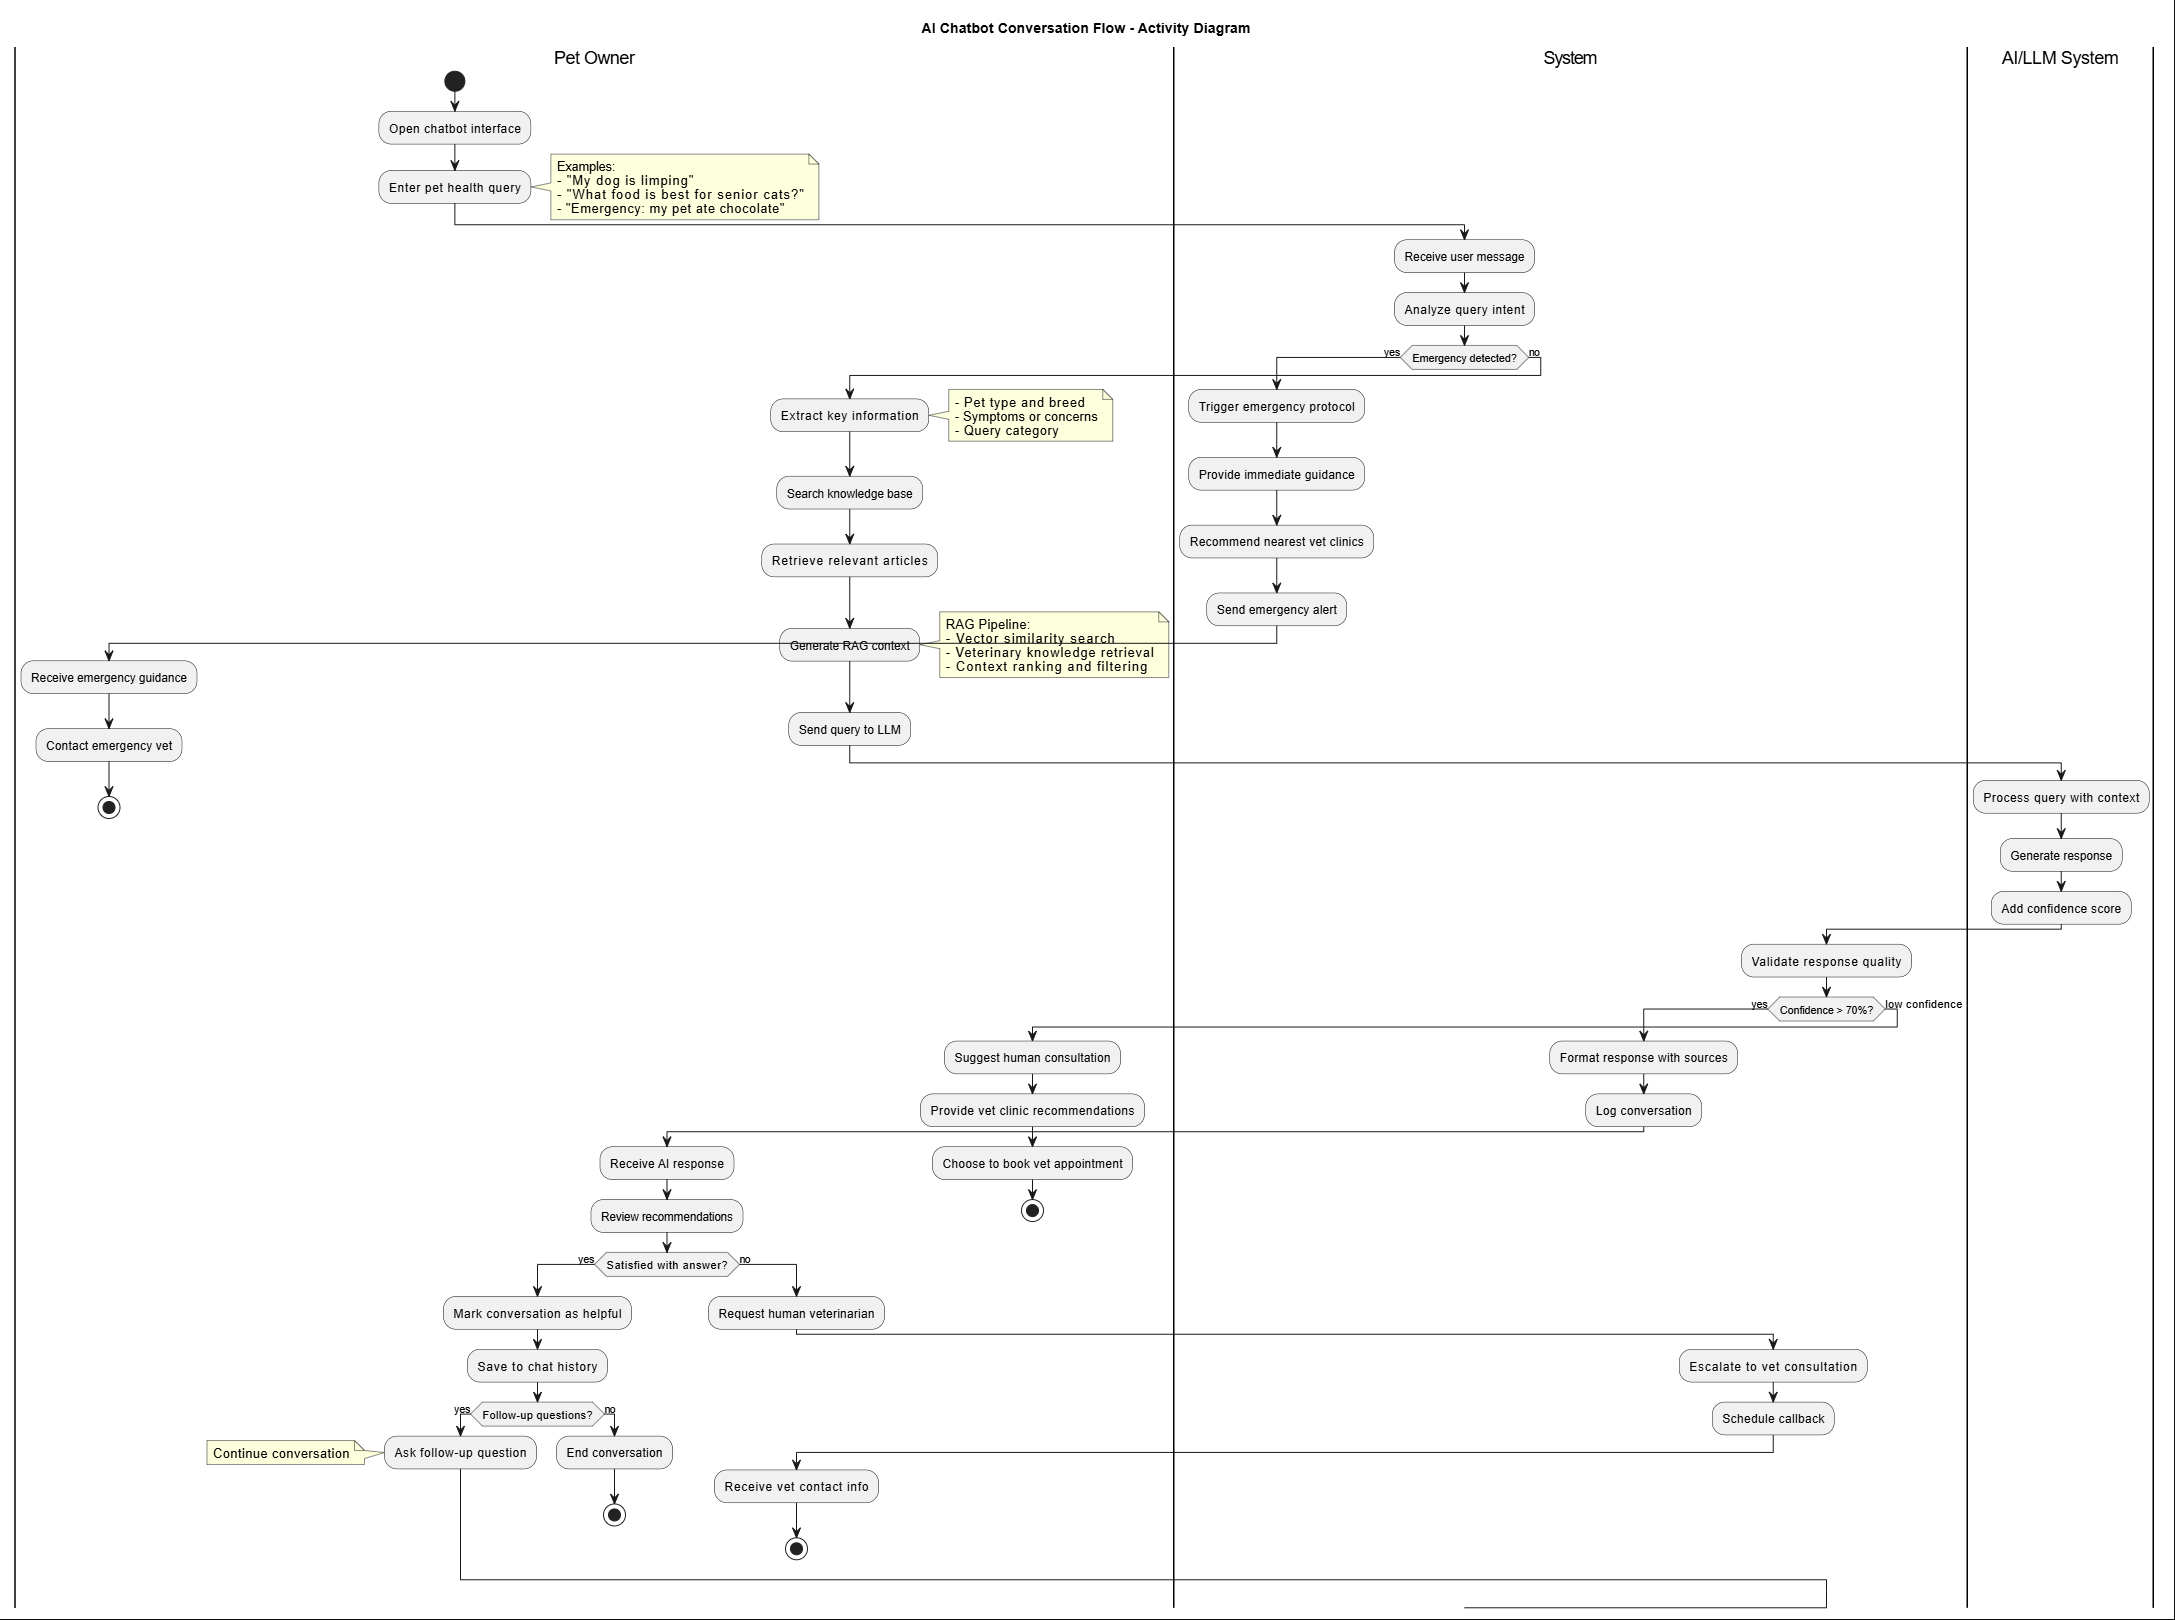
\includegraphics[width=0.9\textwidth]{ThesisFigs/activity_chatbot_conversation.png}
    \caption{Chatbot RAG Query Processing Activity Diagram}
    \label{fig:activity_chatbot}
\end{figure}

User selects pet and types query → backend checks FastAPI availability → HTTP mode: generates embedding → searches ChromaDB (k=2) → constructs prompt → calls Groq API → receives response → checks emergency keywords → displays with alert if urgent → logs conversation.

\subsubsection{Veterinary Appointment Booking}

\begin{figure}[H]
    \centering
    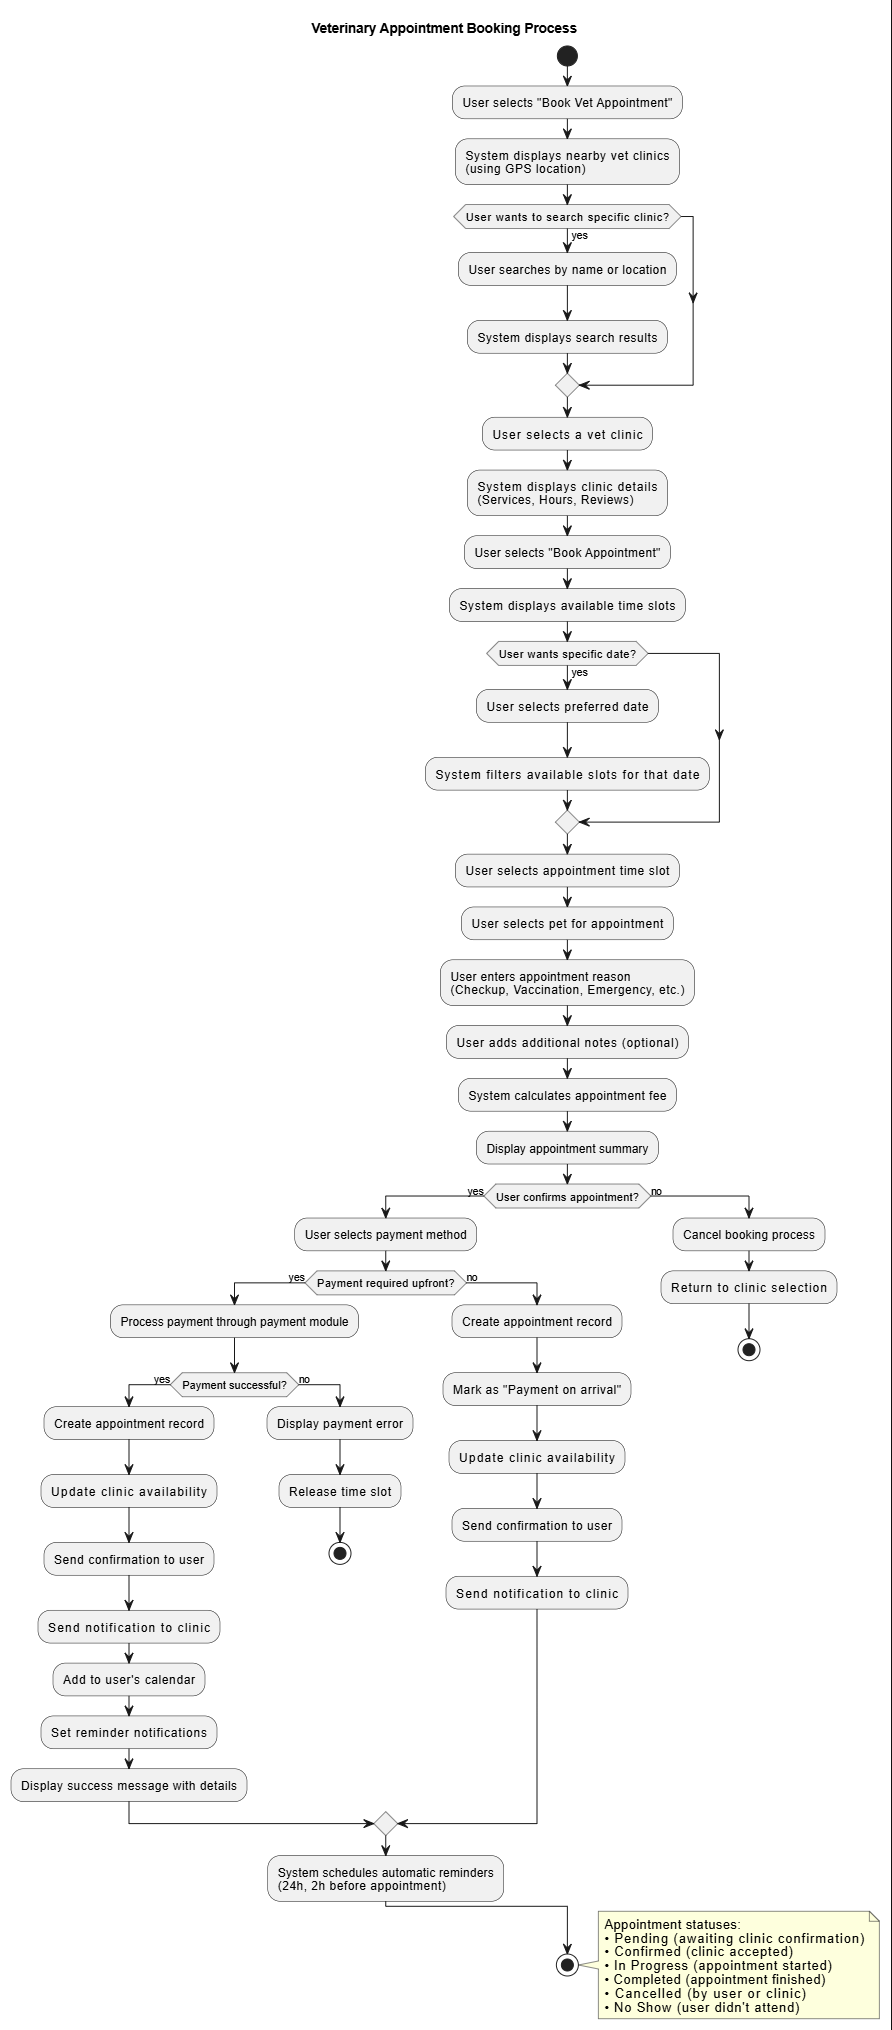
\includegraphics[width=0.9\textwidth]{ThesisFigs/activity_vet_appointment.png}
    \caption{Veterinary Appointment Booking Activity Diagram}
    \label{fig:activity_vet}
\end{figure}

User grants GPS → system queries OpenStreetMap → displays clinics by distance → user selects clinic and date → system shows available slots → user confirms → system creates appointment → sends confirmation → schedules reminders (24h, 2h).

\subsubsection{Health Journal and Vaccination Reminder}

User adds vaccination with due date → system schedules reminder → background job checks daily → 7 days before: sends push notification → user marks completed or reschedules → if completed: updates journal and generates PDF.

\subsection{Class Diagram}

\begin{figure}[H]
    \centering
    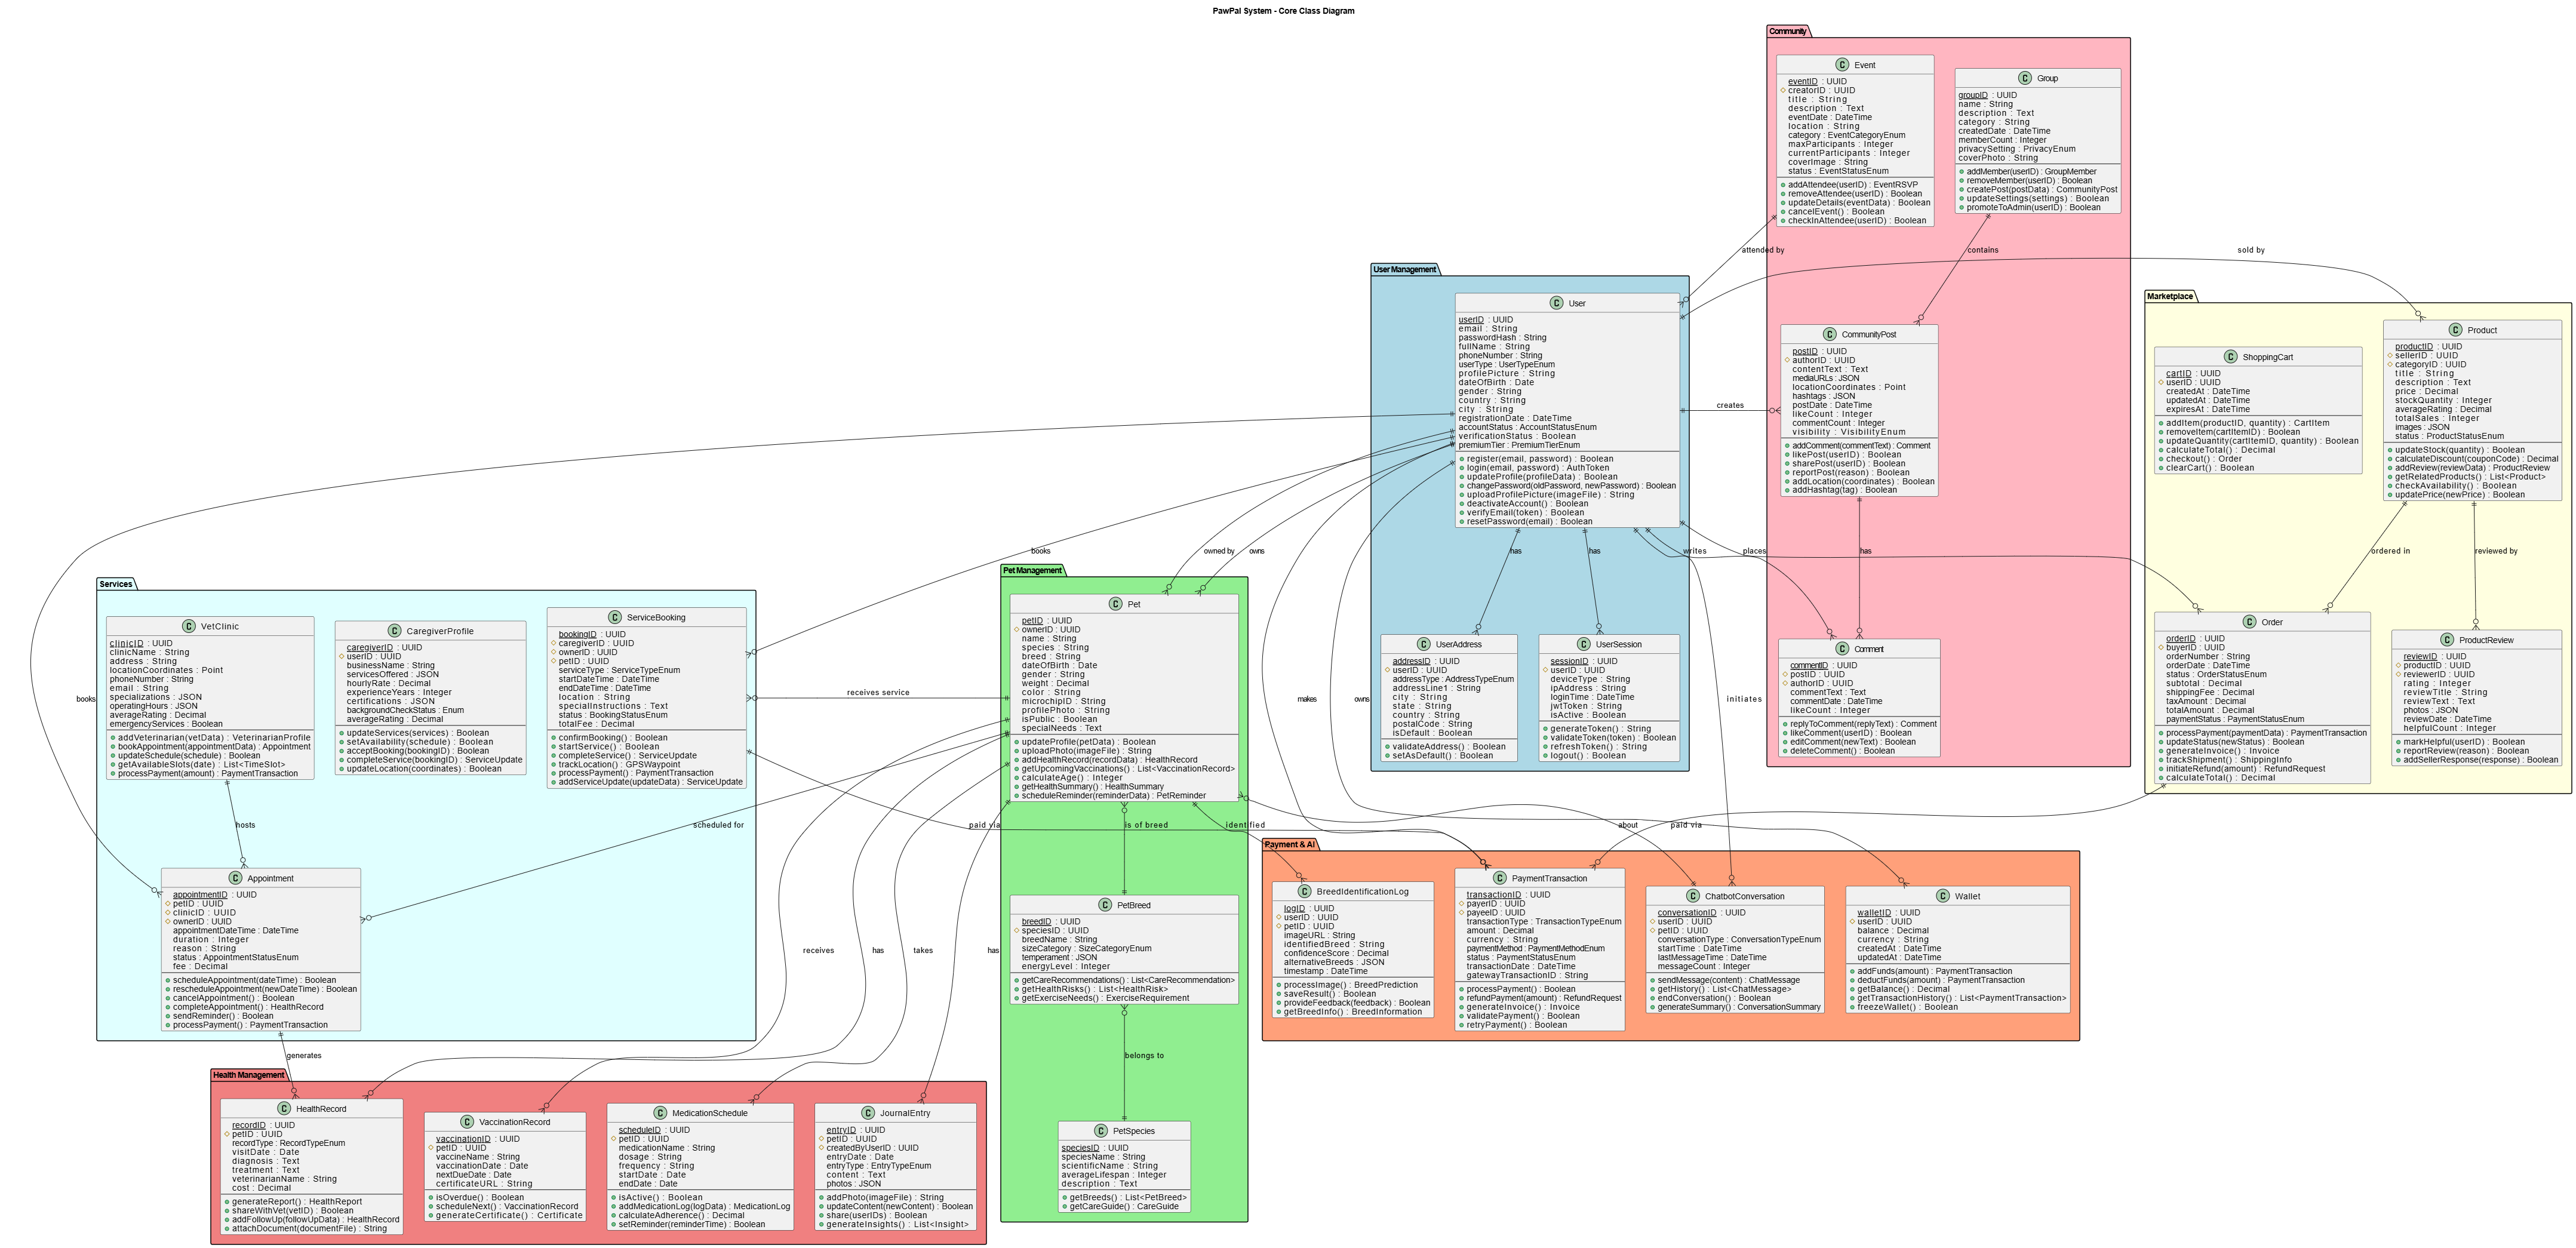
\includegraphics[width=1.0\textwidth]{ThesisFigs/class_diagram.png}
    \caption{PawPal Core Class Diagram}
    \label{fig:class_diagram}
\end{figure}

\textbf{Core Classes:} User (userID, email, passwordHash, name, phone, userType | Register(), Login(), UpdateProfile()), Pet (petID, ownerID, name, species, breed, dob, gender, weight | Create(), Update(), GetHealthJournal() | 1-to-1 HealthJournal), ChatbotService (fastAPIURL, pythonScriptPath, httpClient | Query(), QueryStream(), checkAPIHealth()), BreedIdentificationService (modelEndpoint, imageProcessor | IdentifyBreed(), PreprocessImage(), GetBreedInfo()), Product (productID, sellerID, name, description, price, category, stock | Create(), Update(), AddPhoto() | 1-to-many ProductPhoto max 10), Order (orderID, buyerID, totalAmount, status, paymentMethod | Create(), UpdateStatus(), ProcessPayment(), GenerateInvoice() | composition with OrderItems), Appointment (appointmentID, petOwnerID, veterinarianID, petID, dateTime, status | Book(), Reschedule(), Cancel(), SendReminder() | many-to-1 VeterinaryClinic), PaymentService (cryptoProvider, walletManager | ProcessCryptoPayment(), GenerateQRCode(), MonitorTransaction() | supports Bitcoin/Ethereum/USDT).

\subsection{Sequence Diagrams}

\subsubsection{Chatbot RAG Query with FastAPI}

\begin{figure}[H]
    \centering
    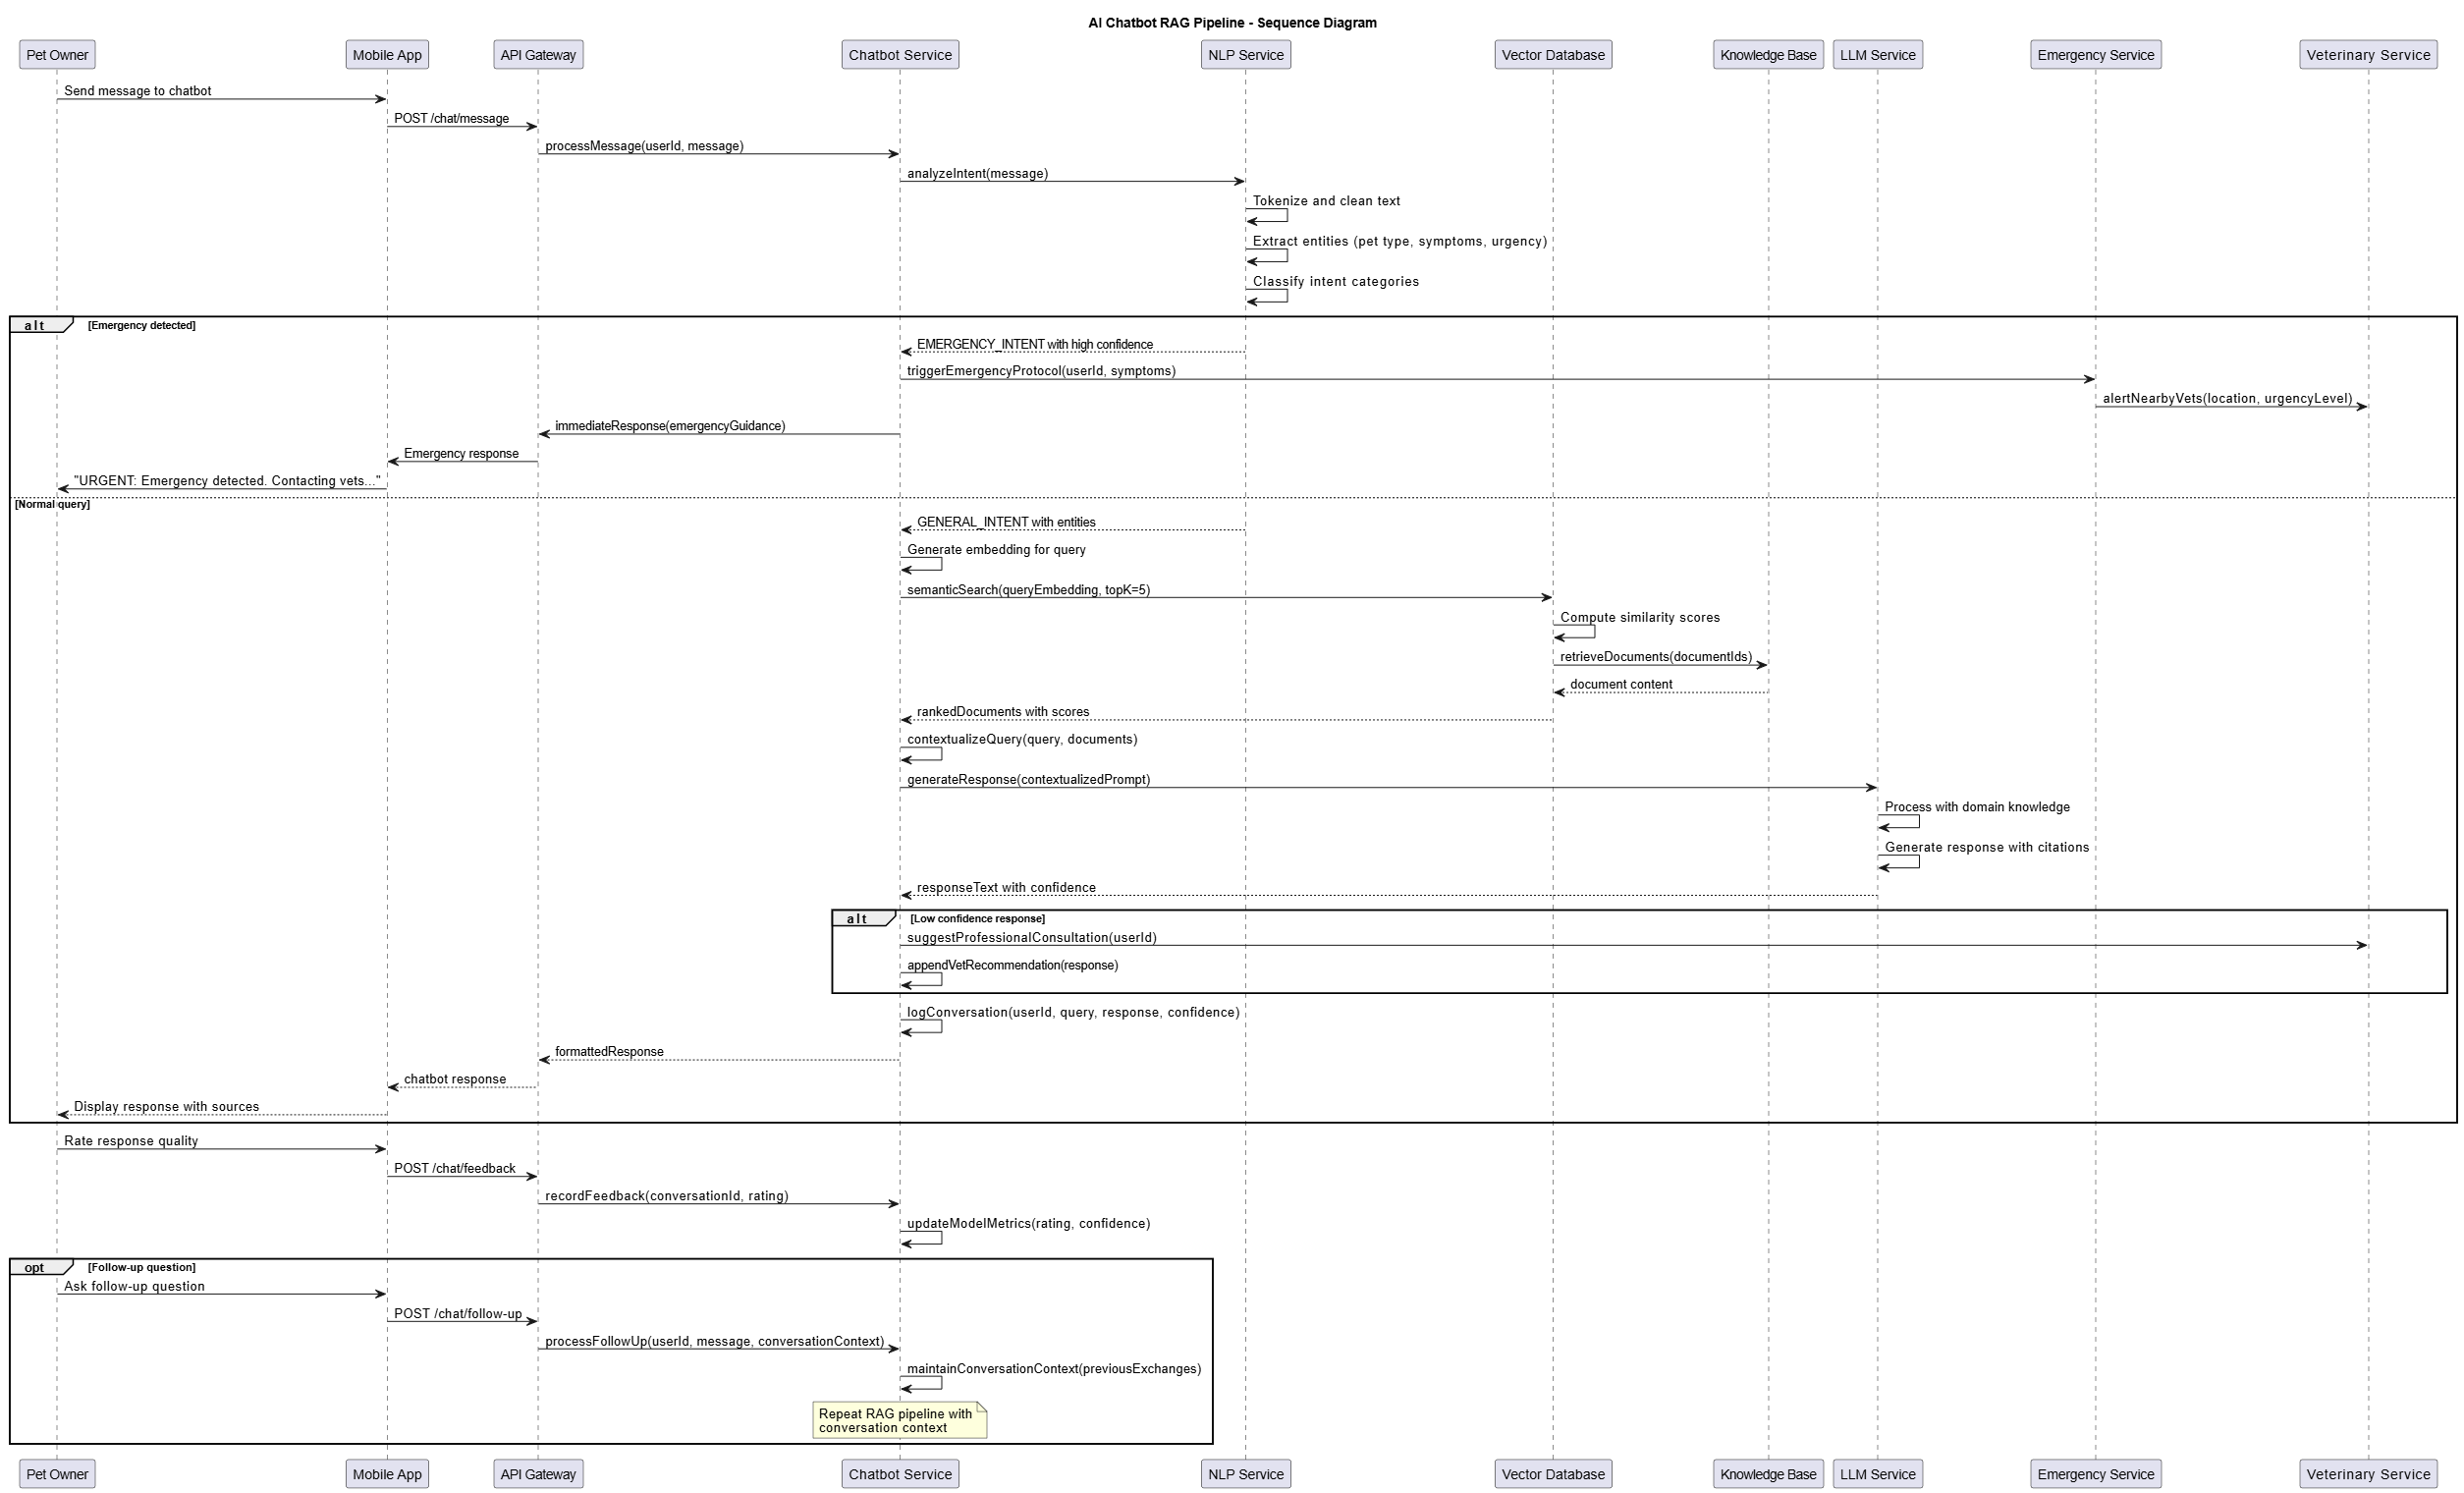
\includegraphics[width=1.0\textwidth]{ThesisFigs/sequence_chatbot_rag_pipeline.png}
    \caption{Chatbot RAG Query Sequence Diagram}
    \label{fig:sequence_chatbot}
\end{figure}

User types query → MobileApp sends POST /api/v1/chatbot/query to GoBackend → GoBackend validates JWT → calls ChatbotService.Query() → checks FastAPI health → sends POST /api/chatbot/query to FastAPIService → FastAPI generates embedding → queries ChromaDB.search(k=2) → retrieves 2 knowledge chunks → constructs prompt with pet context → calls GroqAPI.chat\_completion(max\_tokens=384) → receives LLM response → checks emergency keywords → returns JSON to GoBackend → logs to PostgreSQL → returns to MobileApp → displays response to User.

\subsubsection{Breed Identification with CNN}

\begin{figure}[H]
    \centering
    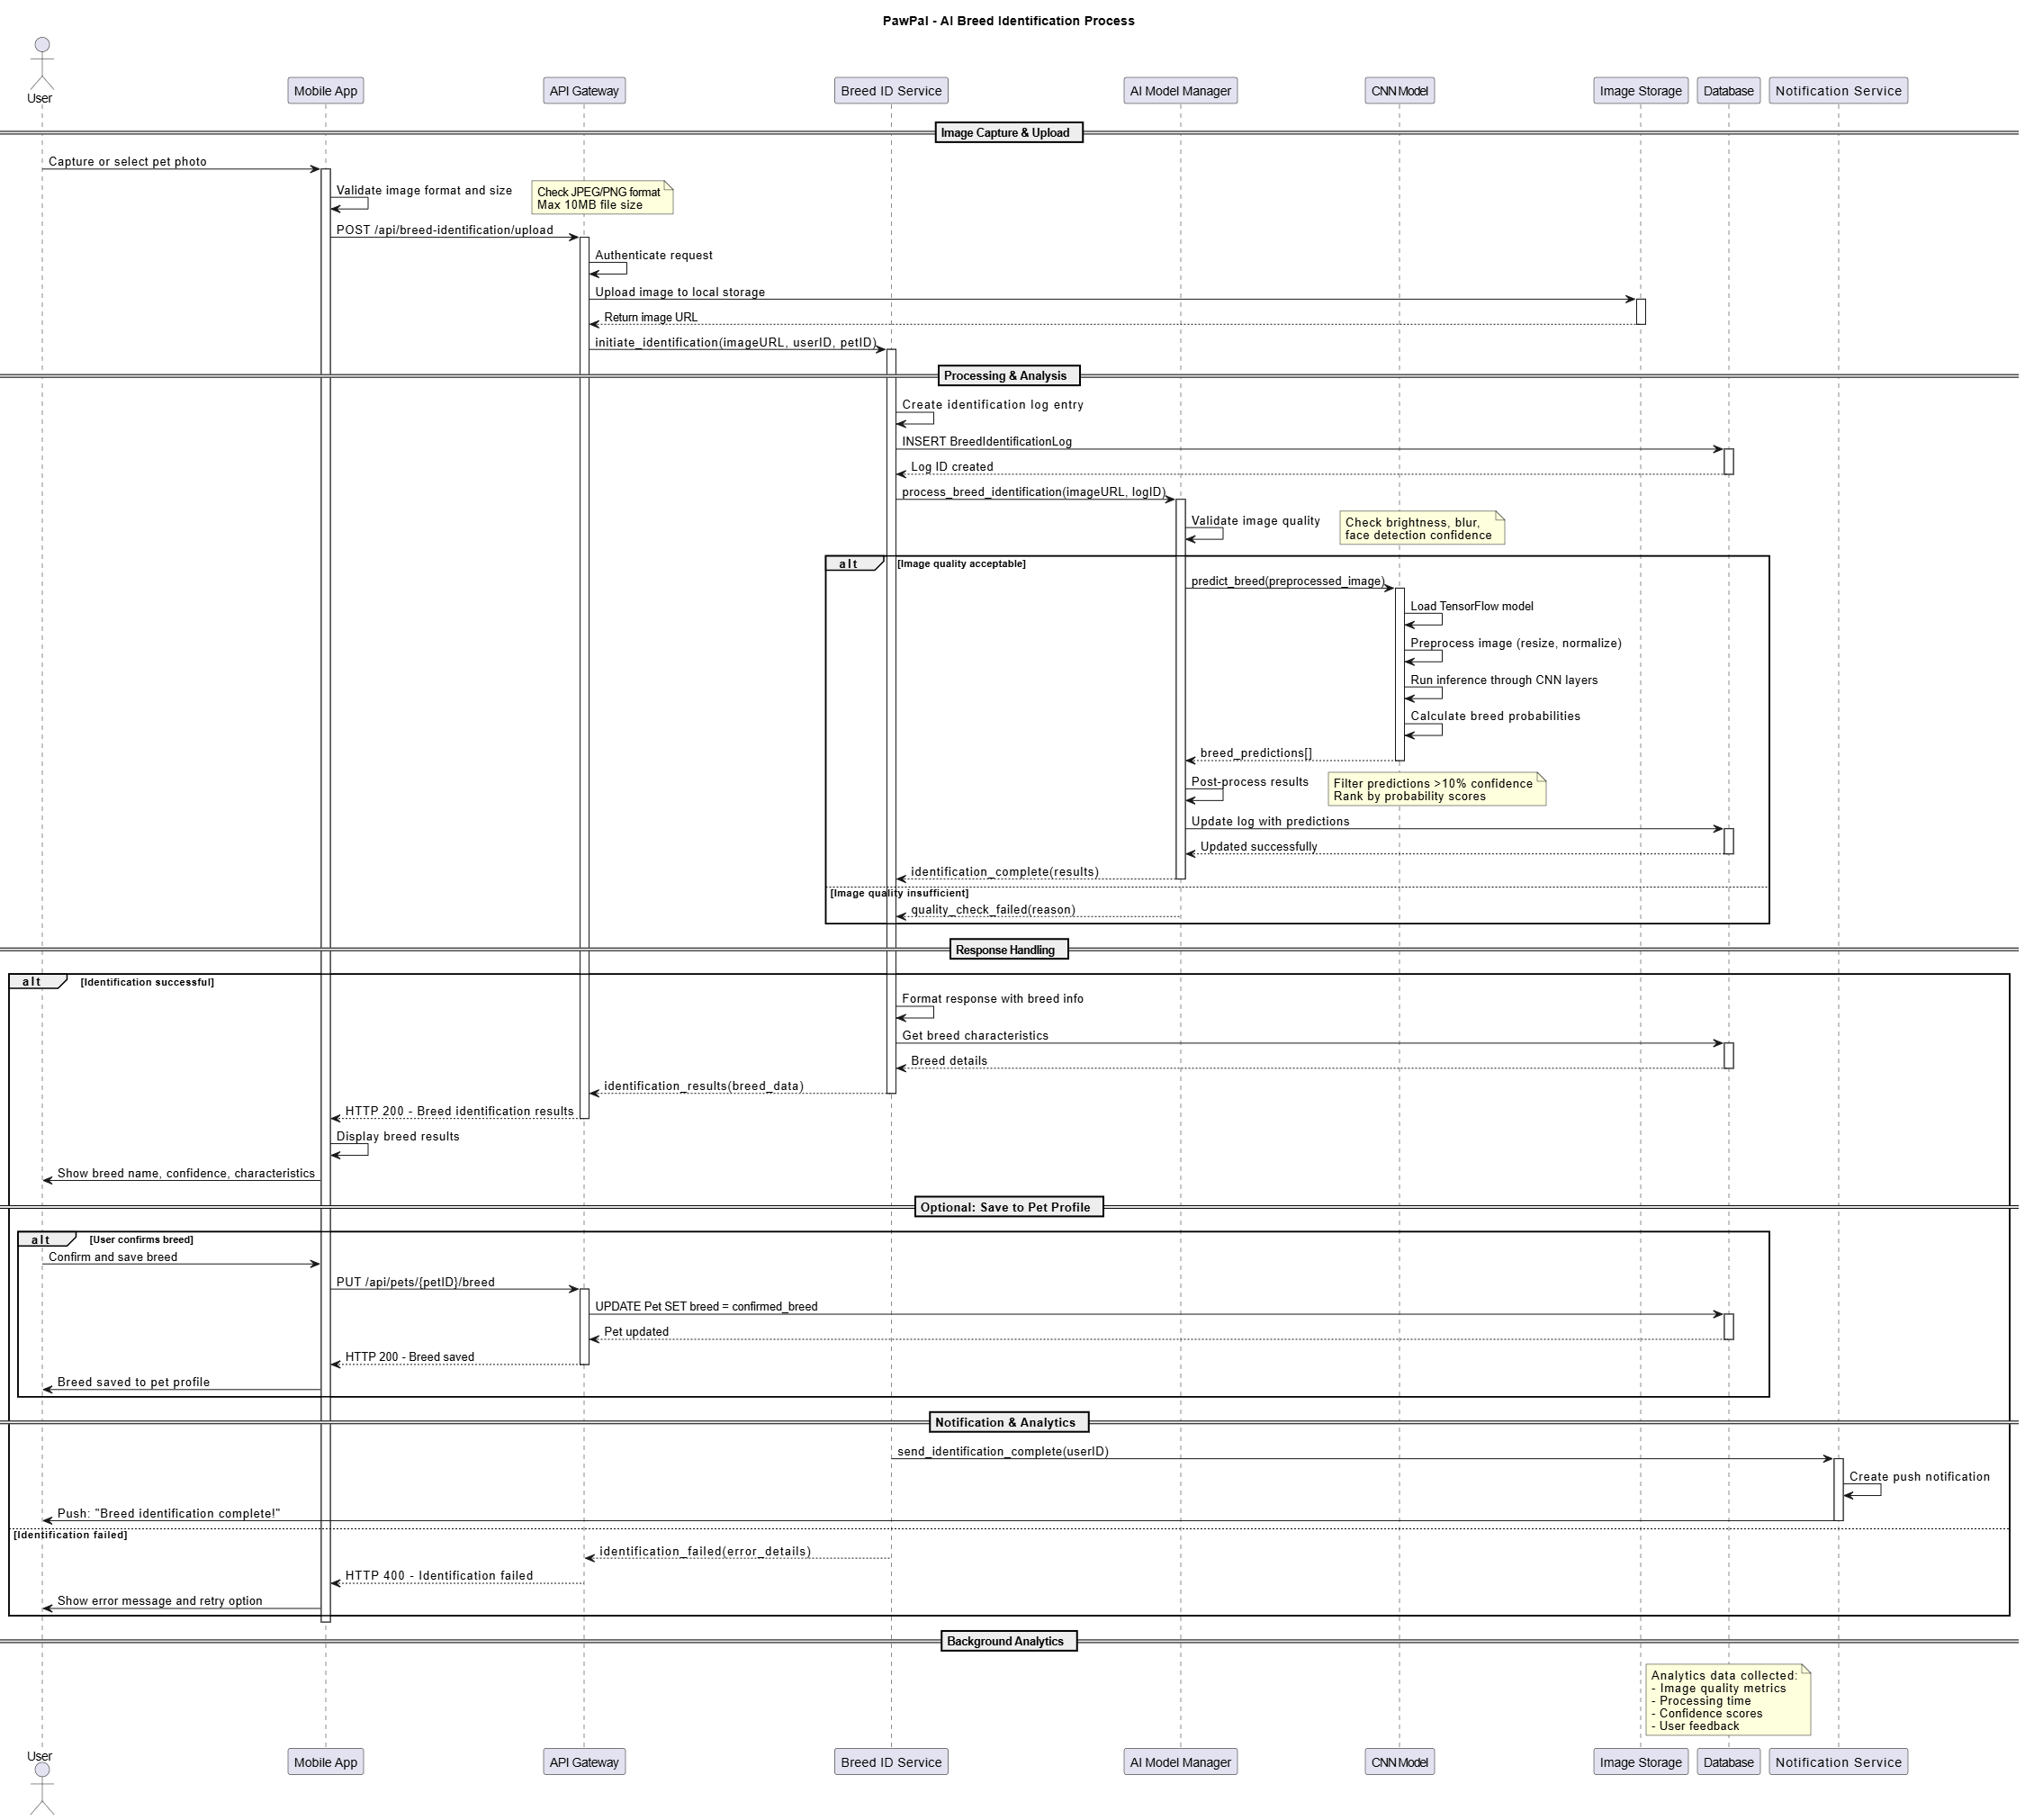
\includegraphics[width=1.0\textwidth]{ThesisFigs/sequence_breed_identification.png}
    \caption{Breed Identification Sequence Diagram}
    \label{fig:sequence_breed}
\end{figure}

User uploads image → MobileApp validates format/size → sends POST /api/v1/pets/identify to GoBackend → calls BreedIdentificationService.IdentifyBreed() → preprocesses (resize 224x224, normalize) → sends to PythonCNNService → loads ConvNeXt V2 model → performs inference → returns top 3 predictions with confidence → GoBackend queries database for breed info → returns predictions + care recommendations → MobileApp displays results.

\subsubsection{Veterinary Appointment with GPS Discovery}

\begin{figure}[H]
    \centering
    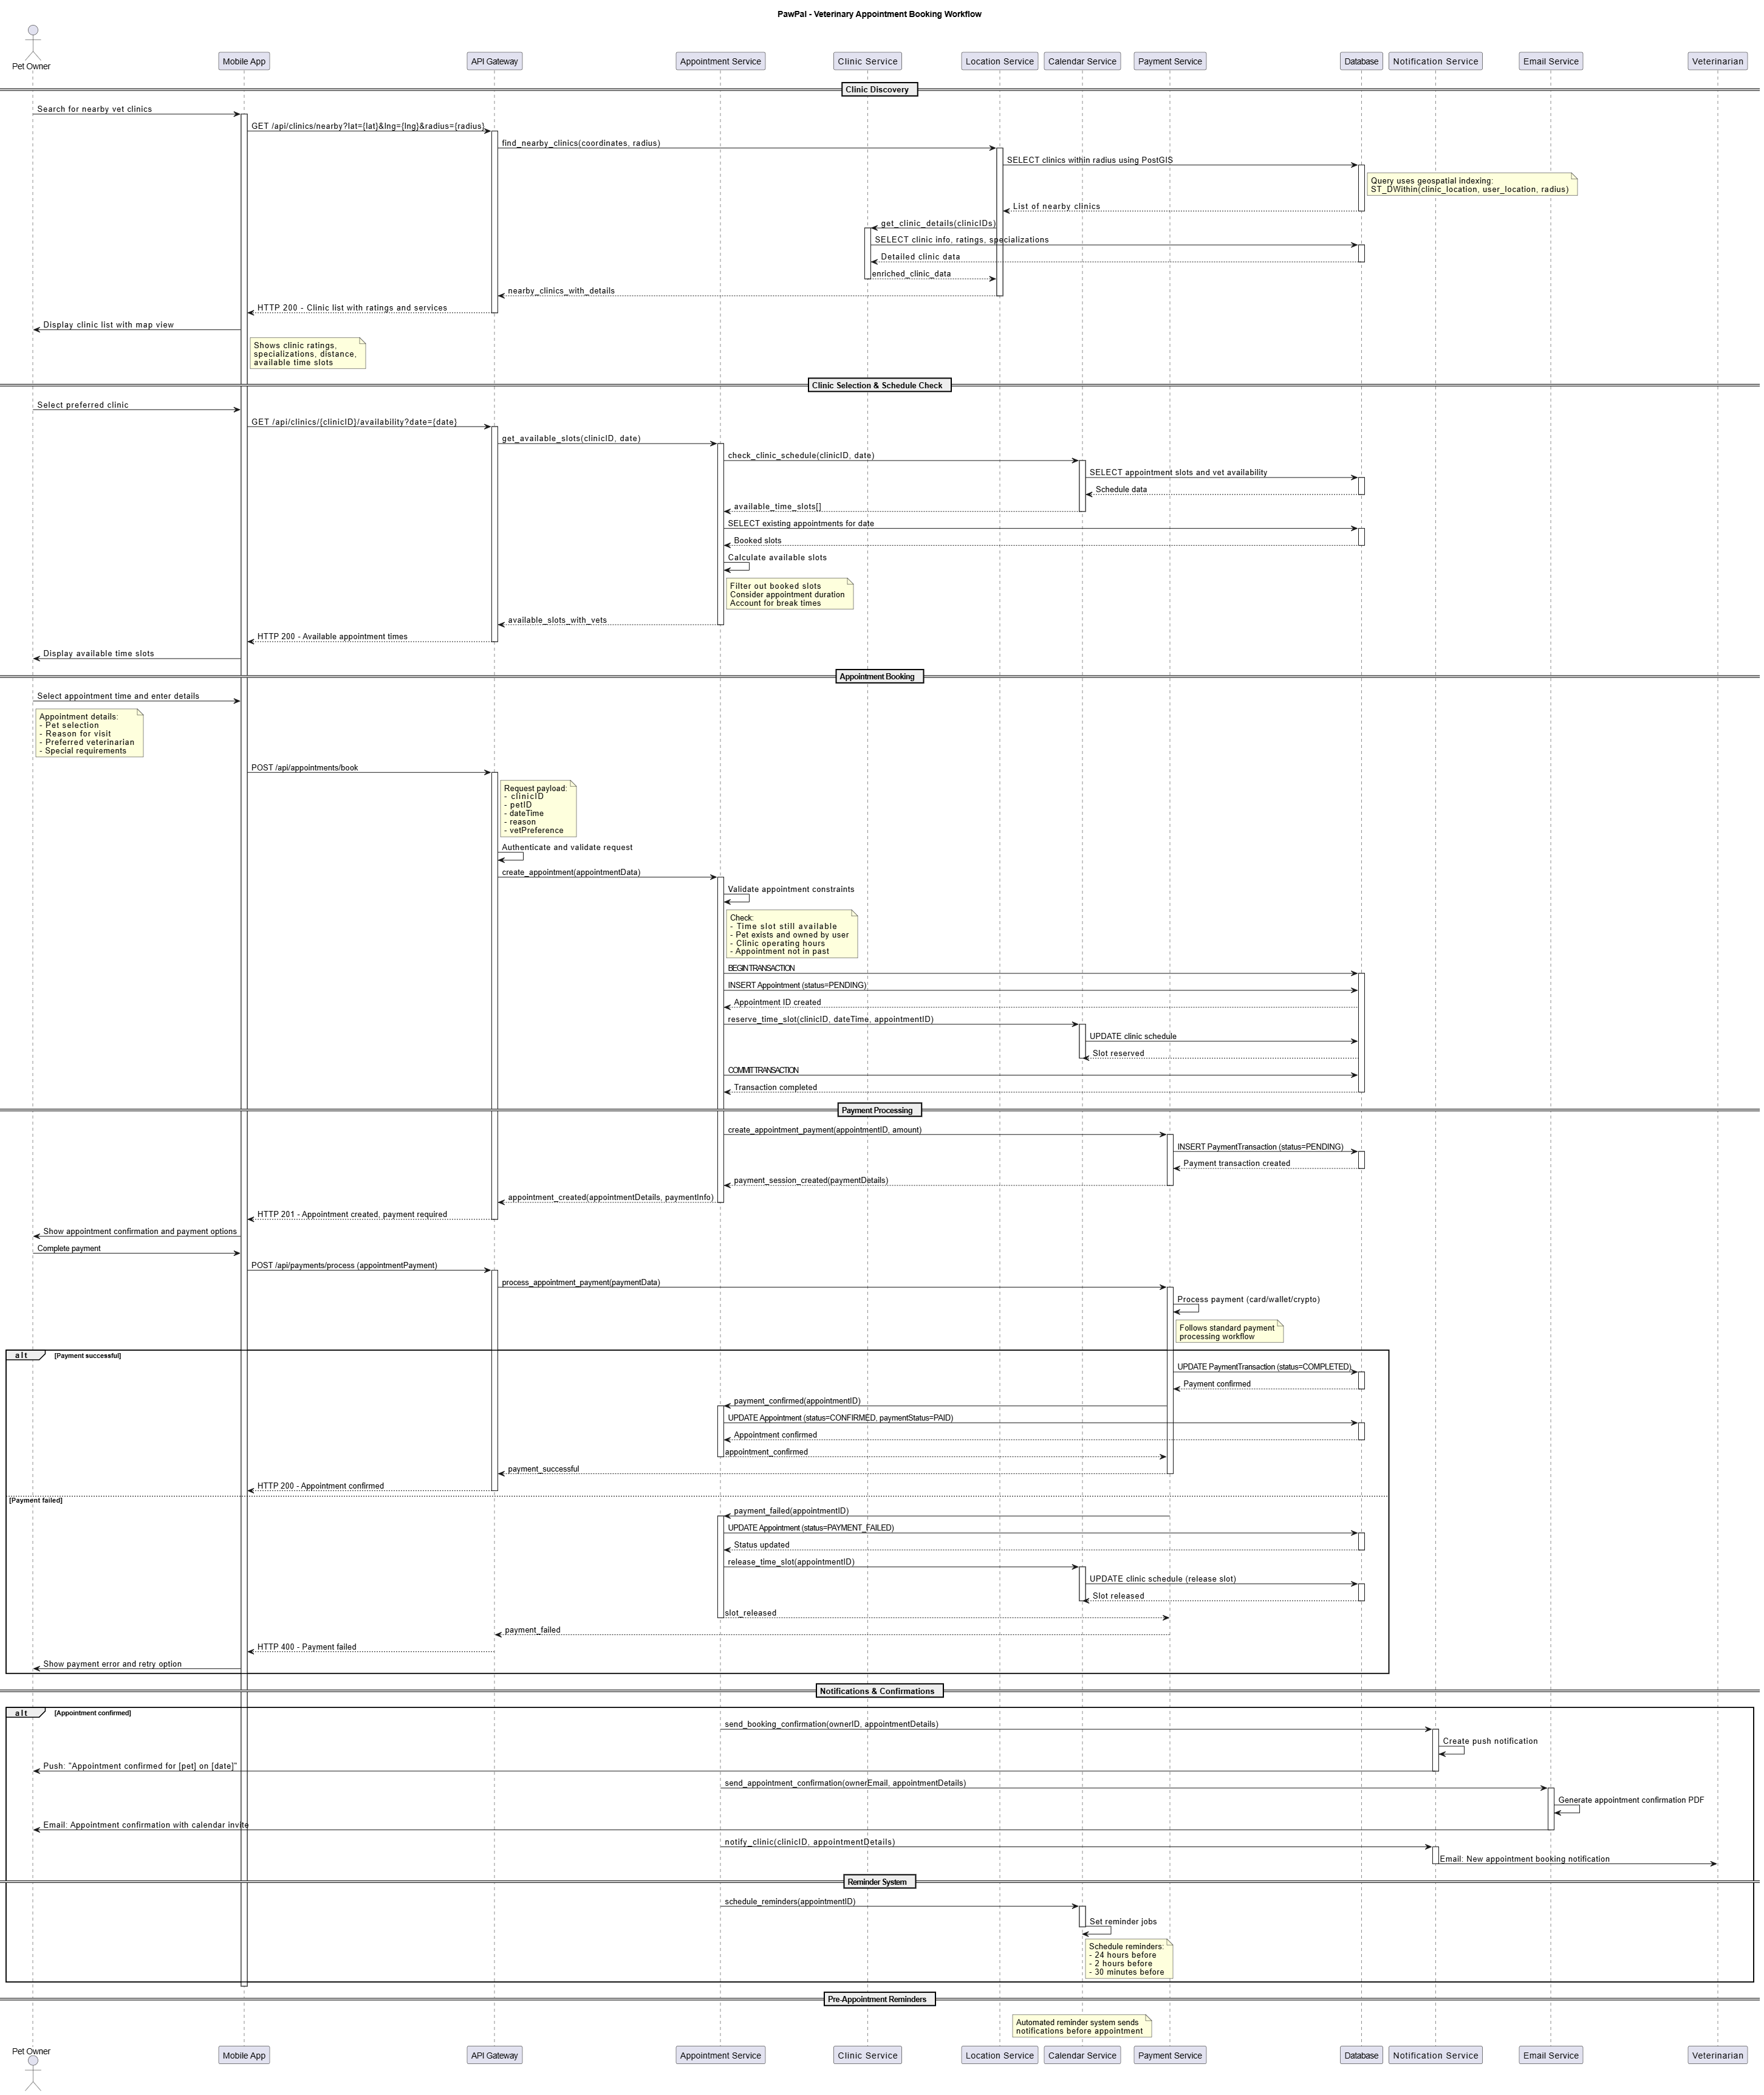
\includegraphics[width=1.0\textwidth]{ThesisFigs/sequence_vet_appointment.png}
    \caption{Veterinary Appointment Sequence Diagram}
    \label{fig:sequence_vet}
\end{figure}

Owner opens Vet Services → MobileApp requests GPS permission → captures coordinates → sends location to GoBackend → queries OpenStreetMapAPI with radius → receives 8 nearby clinics → enriches with database details → MobileApp displays by distance → Owner selects clinic and date → GoBackend queries clinic availability API → receives time slots → Owner confirms slot → GoBackend creates appointment → notifies VeterinaryClinic → schedules reminders in NotificationService → sends confirmation to Owner.

\subsection{State Transition Diagrams}

\subsubsection{Appointment Status Lifecycle}

\begin{figure}[H]
    \centering
    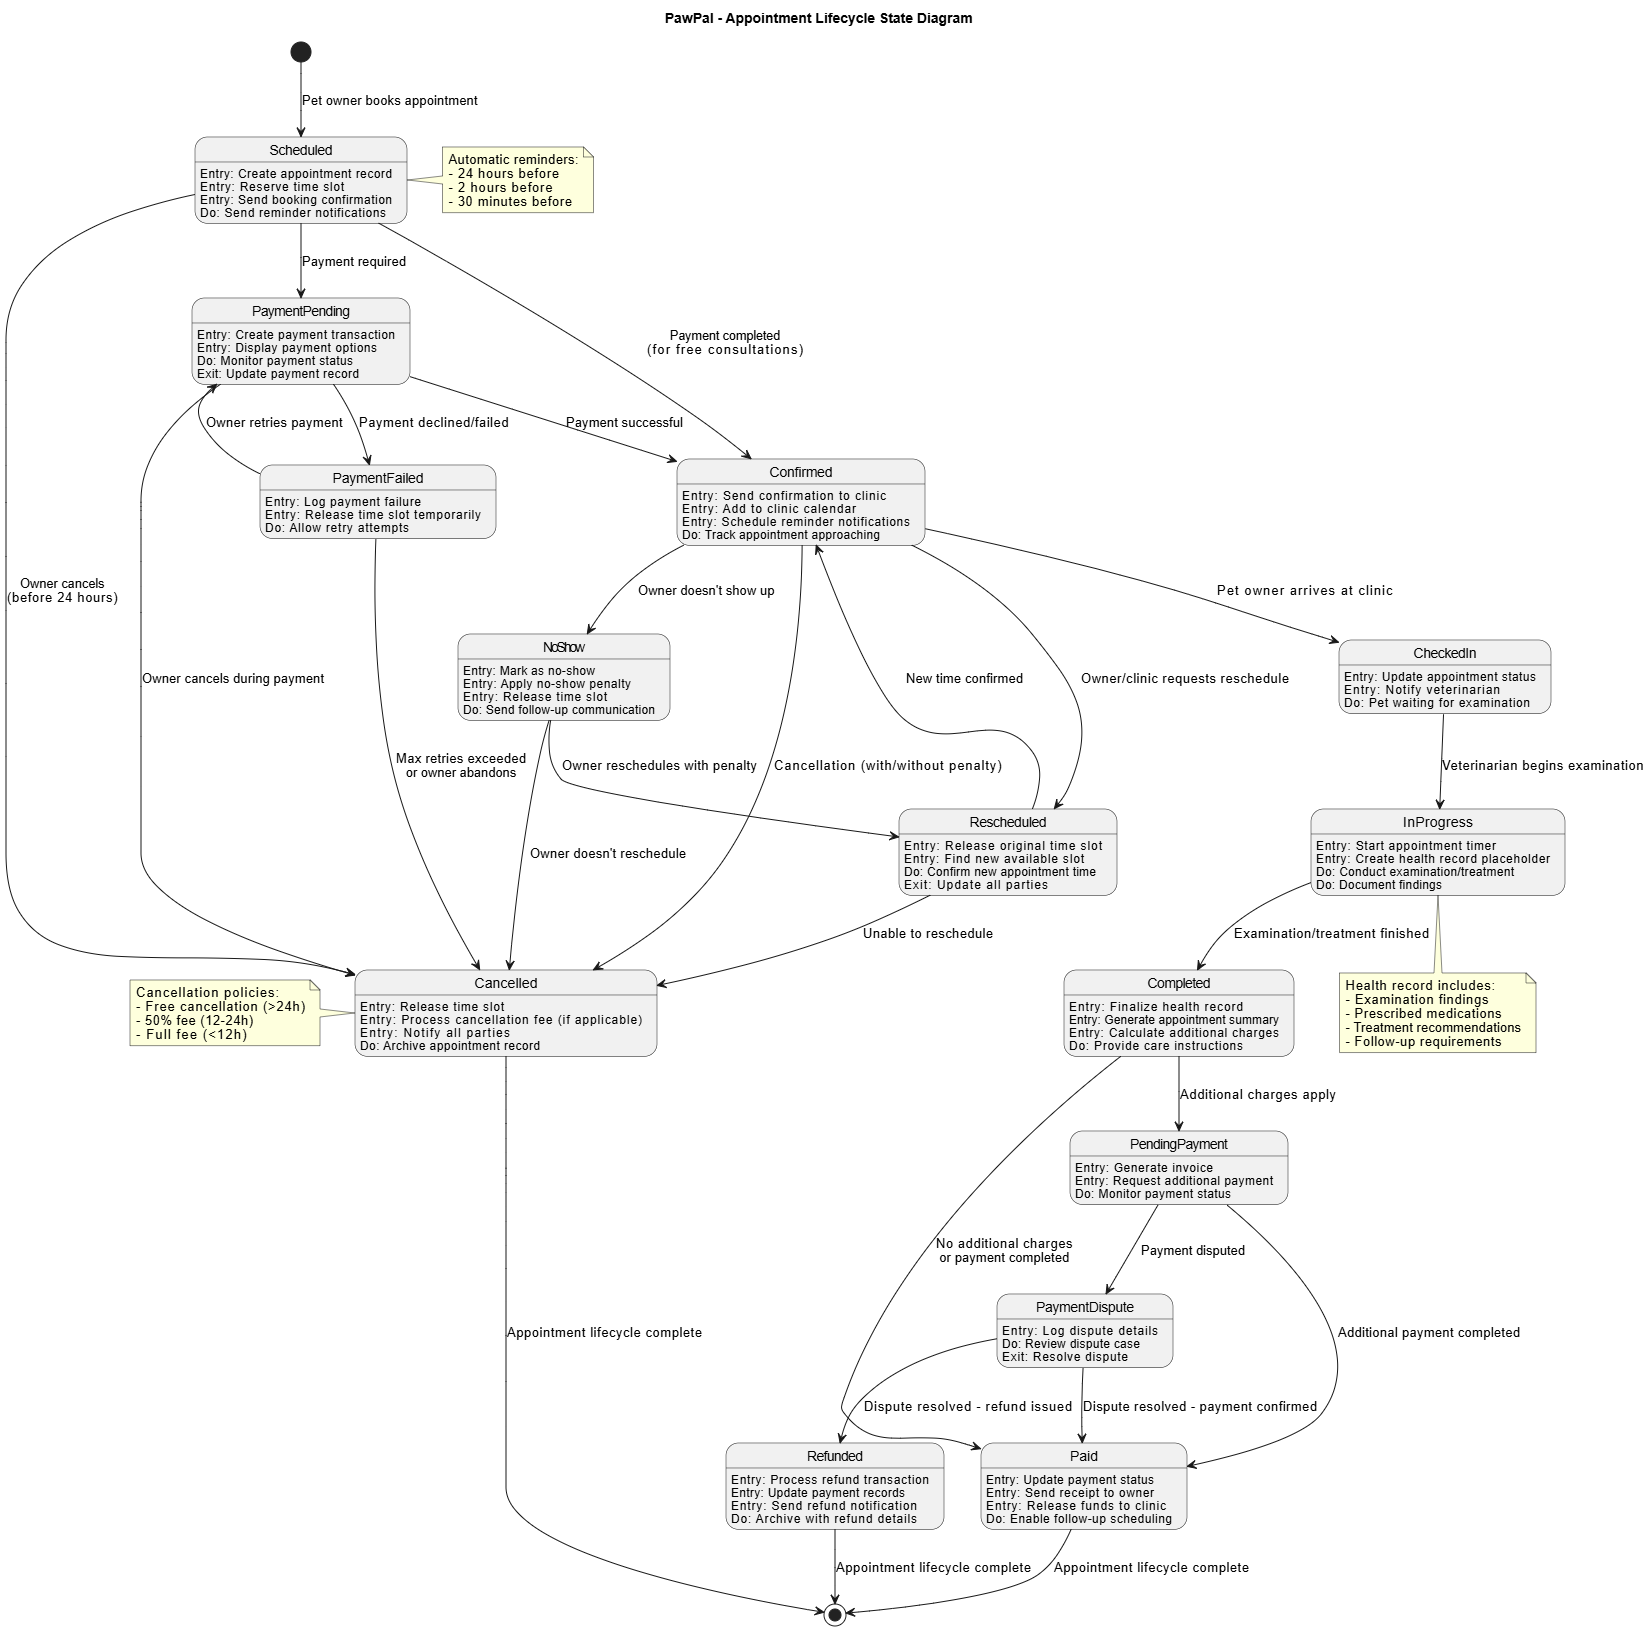
\includegraphics[width=1.0\textwidth]{ThesisFigs/state_appointment_lifecycle.png}
    \caption{Appointment Status Lifecycle State Diagram}
    \label{fig:state_appointment}
\end{figure}

Initial: Requested → Confirmed (vet approves) or Rejected (vet declines). From Confirmed: Rescheduled (owner changes date), Cancelled (owner cancels with 4h+ notice), NoShow (owner misses), or InProgress (appointment starts) → Completed (appointment ends). Final states: Completed, Cancelled, Rejected, NoShow.
